\documentclass[twoside]{book}

% Packages required by doxygen
\usepackage{calc}
\usepackage{doxygen}
\usepackage{graphicx}
\usepackage[utf8]{inputenc}
\usepackage{makeidx}
\usepackage{multicol}
\usepackage{multirow}
\usepackage{textcomp}
\usepackage[table]{xcolor}

% Font selection
\usepackage[T1]{fontenc}
\usepackage{mathptmx}
\usepackage[scaled=.90]{helvet}
\usepackage{courier}
\usepackage{amssymb}
\usepackage{sectsty}
\renewcommand{\familydefault}{\sfdefault}
\allsectionsfont{%
  \fontseries{bc}\selectfont%
  \color{darkgray}%
}
\renewcommand{\DoxyLabelFont}{%
  \fontseries{bc}\selectfont%
  \color{darkgray}%
}

% Page & text layout
\usepackage{geometry}
\geometry{%
  a4paper,%
  top=2.5cm,%
  bottom=2.5cm,%
  left=2.5cm,%
  right=2.5cm%
}
\tolerance=750
\hfuzz=15pt
\hbadness=750
\setlength{\emergencystretch}{15pt}
\setlength{\parindent}{0cm}
\setlength{\parskip}{0.2cm}
\makeatletter
\renewcommand{\paragraph}{%
  \@startsection{paragraph}{4}{0ex}{-1.0ex}{1.0ex}{%
    \normalfont\normalsize\bfseries\SS@parafont%
  }%
}
\renewcommand{\subparagraph}{%
  \@startsection{subparagraph}{5}{0ex}{-1.0ex}{1.0ex}{%
    \normalfont\normalsize\bfseries\SS@subparafont%
  }%
}
\makeatother

% Headers & footers
\usepackage{fancyhdr}
\pagestyle{fancyplain}
\fancyhead[LE]{\fancyplain{}{\bfseries\thepage}}
\fancyhead[CE]{\fancyplain{}{}}
\fancyhead[RE]{\fancyplain{}{\bfseries\leftmark}}
\fancyhead[LO]{\fancyplain{}{\bfseries\rightmark}}
\fancyhead[CO]{\fancyplain{}{}}
\fancyhead[RO]{\fancyplain{}{\bfseries\thepage}}
\fancyfoot[LE]{\fancyplain{}{}}
\fancyfoot[CE]{\fancyplain{}{}}
\fancyfoot[RE]{\fancyplain{}{\bfseries\scriptsize Generated on Wed Mar 12 2014 12:01:21 for Dave by Doxygen }}
\fancyfoot[LO]{\fancyplain{}{\bfseries\scriptsize Generated on Wed Mar 12 2014 12:01:21 for Dave by Doxygen }}
\fancyfoot[CO]{\fancyplain{}{}}
\fancyfoot[RO]{\fancyplain{}{}}
\renewcommand{\footrulewidth}{0.4pt}
\renewcommand{\chaptermark}[1]{%
  \markboth{#1}{}%
}
\renewcommand{\sectionmark}[1]{%
  \markright{\thesection\ #1}%
}

% Indices & bibliography
\usepackage{natbib}
\usepackage[titles]{tocloft}
\setcounter{tocdepth}{3}
\setcounter{secnumdepth}{5}
\makeindex

% Hyperlinks (required, but should be loaded last)
\usepackage{ifpdf}
\ifpdf
  \usepackage[pdftex,pagebackref=true]{hyperref}
\else
  \usepackage[ps2pdf,pagebackref=true]{hyperref}
\fi
\hypersetup{%
  colorlinks=true,%
  linkcolor=blue,%
  citecolor=blue,%
  unicode%
}

% Custom commands
\newcommand{\clearemptydoublepage}{%
  \newpage{\pagestyle{empty}\cleardoublepage}%
}


%===== C O N T E N T S =====

\begin{document}

% Titlepage & ToC
\hypersetup{pageanchor=false}
\pagenumbering{roman}
\begin{titlepage}
\vspace*{7cm}
\begin{center}%
{\Large Dave }\\
\vspace*{1cm}
{\large Generated by Doxygen 1.8.4}\\
\vspace*{0.5cm}
{\small Wed Mar 12 2014 12:01:21}\\
\end{center}
\end{titlepage}
\clearemptydoublepage
\tableofcontents
\clearemptydoublepage
\pagenumbering{arabic}
\hypersetup{pageanchor=true}

%--- Begin generated contents ---
\chapter{Hierarchical Index}
\section{Class Hierarchy}
This inheritance list is sorted roughly, but not completely, alphabetically\-:\begin{DoxyCompactList}
\item \contentsline{section}{Collision}{\pageref{class_collision}}{}
\item Drawable\begin{DoxyCompactList}
\item \contentsline{section}{Game\-Play}{\pageref{class_game_play}}{}
\item \contentsline{section}{Movable}{\pageref{class_movable}}{}
\begin{DoxyCompactList}
\item \contentsline{section}{Collidable}{\pageref{class_collidable}}{}
\begin{DoxyCompactList}
\item \contentsline{section}{Block}{\pageref{class_block}}{}
\item \contentsline{section}{Npc}{\pageref{class_npc}}{}
\item \contentsline{section}{Player}{\pageref{class_player}}{}
\end{DoxyCompactList}
\end{DoxyCompactList}
\end{DoxyCompactList}
\item \contentsline{section}{Vector2\-D}{\pageref{class_vector2_d}}{}
\end{DoxyCompactList}

\chapter{Class Index}
\section{Class List}
Here are the classes, structs, unions and interfaces with brief descriptions\-:\begin{DoxyCompactList}
\item\contentsline{section}{\hyperlink{class_block}{Block} }{\pageref{class_block}}{}
\item\contentsline{section}{\hyperlink{class_collidable}{Collidable} }{\pageref{class_collidable}}{}
\item\contentsline{section}{\hyperlink{class_collision}{Collision} }{\pageref{class_collision}}{}
\item\contentsline{section}{\hyperlink{class_game_play}{Game\-Play} }{\pageref{class_game_play}}{}
\item\contentsline{section}{\hyperlink{class_movable}{Movable} }{\pageref{class_movable}}{}
\item\contentsline{section}{\hyperlink{class_npc}{Npc} }{\pageref{class_npc}}{}
\item\contentsline{section}{\hyperlink{class_player}{Player} }{\pageref{class_player}}{}
\item\contentsline{section}{\hyperlink{class_vector2_d}{Vector2\-D} }{\pageref{class_vector2_d}}{}
\end{DoxyCompactList}

\chapter{File Index}
\section{File List}
Here is a list of all documented files with brief descriptions\-:\begin{DoxyCompactList}
\item\contentsline{section}{include/\hyperlink{_block_8h}{Block.\-h} }{\pageref{_block_8h}}{}
\item\contentsline{section}{include/\hyperlink{_collidable_8h}{Collidable.\-h} }{\pageref{_collidable_8h}}{}
\item\contentsline{section}{include/\hyperlink{_collision_8h}{Collision.\-h} }{\pageref{_collision_8h}}{}
\item\contentsline{section}{include/\hyperlink{_game_play_8h}{Game\-Play.\-h} }{\pageref{_game_play_8h}}{}
\item\contentsline{section}{include/\hyperlink{_movable_8h}{Movable.\-h} }{\pageref{_movable_8h}}{}
\item\contentsline{section}{include/\hyperlink{_npc_8h}{Npc.\-h} }{\pageref{_npc_8h}}{}
\item\contentsline{section}{include/\hyperlink{_player_8h}{Player.\-h} }{\pageref{_player_8h}}{}
\item\contentsline{section}{include/\hyperlink{_vector2_d_8h}{Vector2\-D.\-h} }{\pageref{_vector2_d_8h}}{}
\item\contentsline{section}{src/\hyperlink{_collidable_8cpp}{Collidable.\-cpp} }{\pageref{_collidable_8cpp}}{}
\item\contentsline{section}{src/\hyperlink{_game_play_8cpp}{Game\-Play.\-cpp} }{\pageref{_game_play_8cpp}}{}
\item\contentsline{section}{src/\hyperlink{_movable_8cpp}{Movable.\-cpp} }{\pageref{_movable_8cpp}}{}
\item\contentsline{section}{src/\hyperlink{_player_8cpp}{Player.\-cpp} }{\pageref{_player_8cpp}}{}
\item\contentsline{section}{src/\hyperlink{_vector2_d_8cpp}{Vector2\-D.\-cpp} }{\pageref{_vector2_d_8cpp}}{}
\end{DoxyCompactList}

\chapter{Class Documentation}
\hypertarget{class_block}{\section{Block Class Reference}
\label{class_block}\index{Block@{Block}}
}


{\ttfamily \#include $<$Block.\-h$>$}

Inheritance diagram for Block\-:\begin{figure}[H]
\begin{center}
\leavevmode
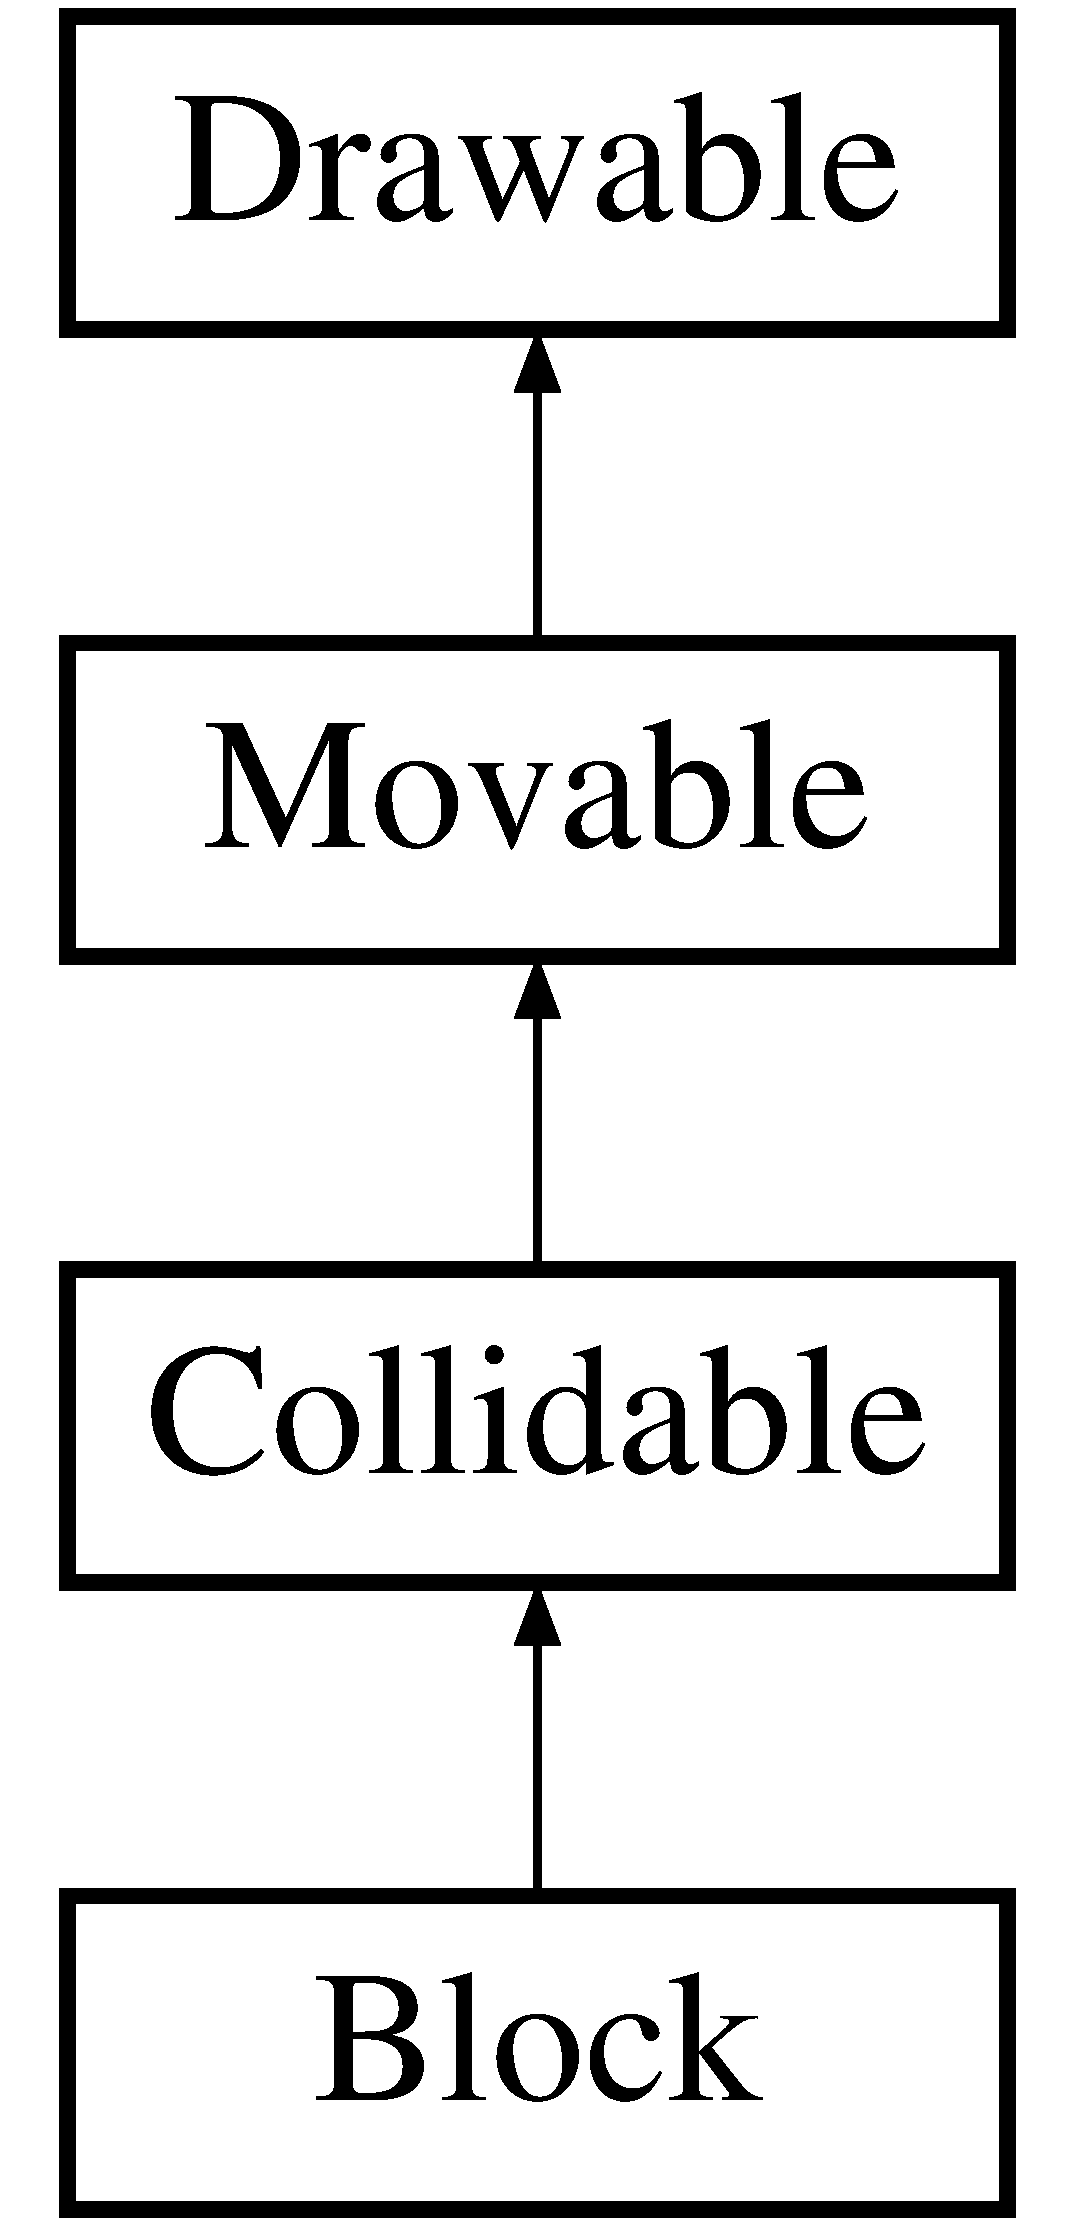
\includegraphics[height=4.000000cm]{class_block}
\end{center}
\end{figure}
\subsection*{Public Member Functions}
\begin{DoxyCompactItemize}
\item 
\hypertarget{class_block_a37658a946bf5067ad01d68d9ff086adc}{\hyperlink{class_block_a37658a946bf5067ad01d68d9ff086adc}{Block} ()}\label{class_block_a37658a946bf5067ad01d68d9ff086adc}

\begin{DoxyCompactList}\small\item\em default constructor \end{DoxyCompactList}\item 
void \hyperlink{class_block_a807c16fcd68933c3a82c4b66c967bc8c}{set\-Block} (int n, float x\-Pos, float y\-Pos, sf\-::\-Texture \&t)
\begin{DoxyCompactList}\small\item\em set type of block \end{DoxyCompactList}\item 
void \hyperlink{class_block_ab21be2cadeac40c67633643f3b04977a}{set\-Special} (bool s)
\begin{DoxyCompactList}\small\item\em set if block is special \end{DoxyCompactList}\item 
void \hyperlink{class_block_a16fe4b0dc9c8f27c28470e8344e5d83a}{set\-Hits} (int h)
\begin{DoxyCompactList}\small\item\em set amounts of hits a destroyable block can take \end{DoxyCompactList}\item 
void \hyperlink{class_block_aed9186020707930f3802e63421cc5ee0}{set\-Used} (bool u)
\begin{DoxyCompactList}\small\item\em set if the block has been hit or not \end{DoxyCompactList}\item 
\hypertarget{class_block_a53401ddc379be16706e26b32b28d2272}{int \hyperlink{class_block_a53401ddc379be16706e26b32b28d2272}{get\-Hits} ()}\label{class_block_a53401ddc379be16706e26b32b28d2272}

\begin{DoxyCompactList}\small\item\em return amount of hits left on a block \end{DoxyCompactList}\item 
\hypertarget{class_block_acdbaef798dfa2a7f65091d161bee908e}{bool \hyperlink{class_block_acdbaef798dfa2a7f65091d161bee908e}{get\-Special} ()}\label{class_block_acdbaef798dfa2a7f65091d161bee908e}

\begin{DoxyCompactList}\small\item\em return if the block is special or not \end{DoxyCompactList}\item 
\hypertarget{class_block_ae3dcd52cb3fbbfa2ffd1d9fd4e6e2b41}{bool \hyperlink{class_block_ae3dcd52cb3fbbfa2ffd1d9fd4e6e2b41}{get\-Used} ()}\label{class_block_ae3dcd52cb3fbbfa2ffd1d9fd4e6e2b41}

\begin{DoxyCompactList}\small\item\em returns if the special block has been hit by player or not \end{DoxyCompactList}\end{DoxyCompactItemize}
\subsection*{Friends}
\begin{DoxyCompactItemize}
\item 
\hypertarget{class_block_a580bc16a3fc18eb382fed53c6a31c365}{class {\bfseries Movable}}\label{class_block_a580bc16a3fc18eb382fed53c6a31c365}

\end{DoxyCompactItemize}
\subsection*{Additional Inherited Members}


\subsection{Detailed Description}
class for the level 

\subsection{Member Function Documentation}
\hypertarget{class_block_a807c16fcd68933c3a82c4b66c967bc8c}{\index{Block@{Block}!set\-Block@{set\-Block}}
\index{set\-Block@{set\-Block}!Block@{Block}}
\subsubsection[{set\-Block}]{\setlength{\rightskip}{0pt plus 5cm}void Block\-::set\-Block (
\begin{DoxyParamCaption}
\item[{int}]{n, }
\item[{float}]{x\-Pos, }
\item[{float}]{y\-Pos, }
\item[{sf\-::\-Texture \&}]{t}
\end{DoxyParamCaption}
)}}\label{class_block_a807c16fcd68933c3a82c4b66c967bc8c}


set type of block 

set image properties (all blocks same size)

Checks value entered in function and creates a block depending on the integer value 
\begin{DoxyParams}{Parameters}
{\em t} & set block function \\
\hline
\end{DoxyParams}
\hypertarget{class_block_a16fe4b0dc9c8f27c28470e8344e5d83a}{\index{Block@{Block}!set\-Hits@{set\-Hits}}
\index{set\-Hits@{set\-Hits}!Block@{Block}}
\subsubsection[{set\-Hits}]{\setlength{\rightskip}{0pt plus 5cm}void Block\-::set\-Hits (
\begin{DoxyParamCaption}
\item[{int}]{h}
\end{DoxyParamCaption}
)}}\label{class_block_a16fe4b0dc9c8f27c28470e8344e5d83a}


set amounts of hits a destroyable block can take 


\begin{DoxyParams}{Parameters}
{\em h} & set hits for block \\
\hline
\end{DoxyParams}
\hypertarget{class_block_ab21be2cadeac40c67633643f3b04977a}{\index{Block@{Block}!set\-Special@{set\-Special}}
\index{set\-Special@{set\-Special}!Block@{Block}}
\subsubsection[{set\-Special}]{\setlength{\rightskip}{0pt plus 5cm}void Block\-::set\-Special (
\begin{DoxyParamCaption}
\item[{bool}]{s}
\end{DoxyParamCaption}
)}}\label{class_block_ab21be2cadeac40c67633643f3b04977a}


set if block is special 


\begin{DoxyParams}{Parameters}
{\em s} & set if the block is special \\
\hline
\end{DoxyParams}
\hypertarget{class_block_aed9186020707930f3802e63421cc5ee0}{\index{Block@{Block}!set\-Used@{set\-Used}}
\index{set\-Used@{set\-Used}!Block@{Block}}
\subsubsection[{set\-Used}]{\setlength{\rightskip}{0pt plus 5cm}void Block\-::set\-Used (
\begin{DoxyParamCaption}
\item[{bool}]{u}
\end{DoxyParamCaption}
)}}\label{class_block_aed9186020707930f3802e63421cc5ee0}


set if the block has been hit or not 


\begin{DoxyParams}{Parameters}
{\em u} & set if the block has been hit \\
\hline
\end{DoxyParams}


The documentation for this class was generated from the following files\-:\begin{DoxyCompactItemize}
\item 
include/\hyperlink{_block_8h}{Block.\-h}\item 
src/Block.\-cpp\end{DoxyCompactItemize}

\hypertarget{class_collidable}{\section{Collidable Class Reference}
\label{class_collidable}\index{Collidable@{Collidable}}
}


{\ttfamily \#include $<$Collidable.\-h$>$}

Inheritance diagram for Collidable\-:\begin{figure}[H]
\begin{center}
\leavevmode
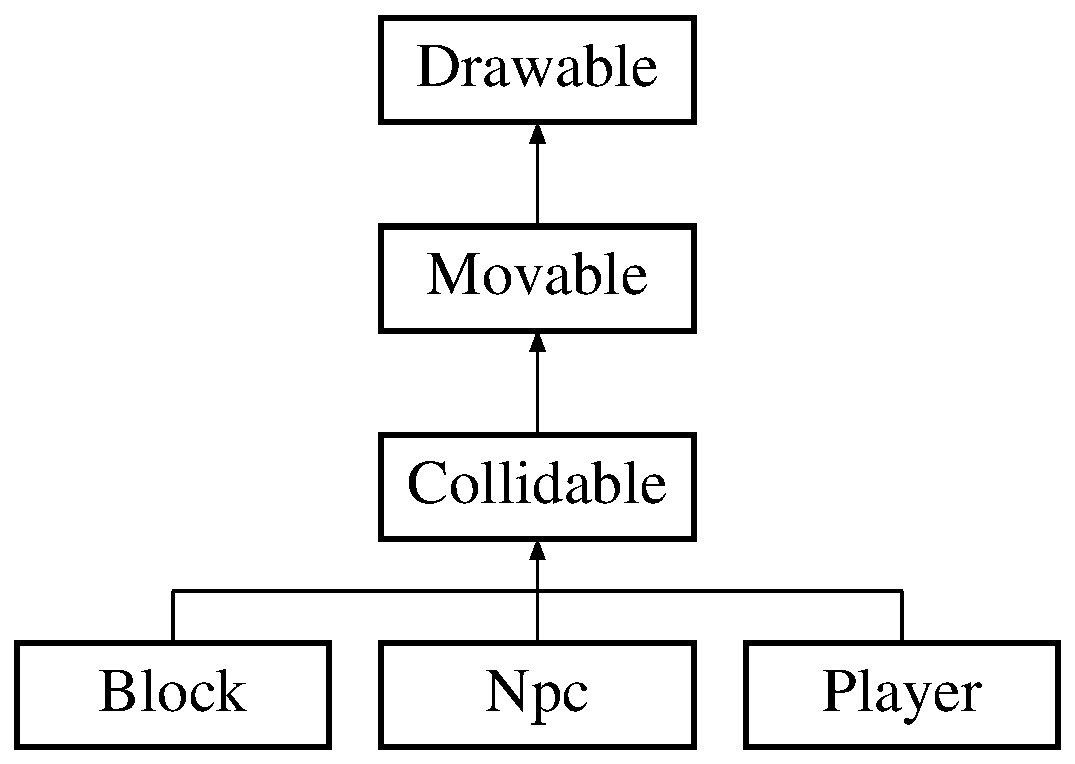
\includegraphics[height=4.000000cm]{class_collidable}
\end{center}
\end{figure}
\subsection*{Public Member Functions}
\begin{DoxyCompactItemize}
\item 
\hypertarget{class_collidable_a92ce9e2b08086bb2f466168ffc69c9ed}{\hyperlink{class_collidable_a92ce9e2b08086bb2f466168ffc69c9ed}{Collidable} ()}\label{class_collidable_a92ce9e2b08086bb2f466168ffc69c9ed}

\begin{DoxyCompactList}\small\item\em default constructor \end{DoxyCompactList}\item 
void \hyperlink{class_collidable_ae65b7398b66bdc89bef21ec9643ac0ff}{set\-Size} (\hyperlink{class_vector2_d}{Vector2\-D} \&s)
\begin{DoxyCompactList}\small\item\em set size of object \end{DoxyCompactList}\item 
void \hyperlink{class_collidable_a8d6d8c505ce98690d38f569a8643e530}{seti\-Mass} (float i\-M)
\begin{DoxyCompactList}\small\item\em set inverse mass of object \end{DoxyCompactList}\item 
void \hyperlink{class_collidable_ab47021e982cc06470e49a0e69d2c9b87}{set\-Elasticity} (float e)
\begin{DoxyCompactList}\small\item\em set elasticity of object \end{DoxyCompactList}\item 
void \hyperlink{class_collidable_a0632214472cc5139d932310b2407ffdb}{set\-Normal} (\hyperlink{class_vector2_d}{Vector2\-D} \&n)
\begin{DoxyCompactList}\small\item\em set the normal of the object \end{DoxyCompactList}\item 
void \hyperlink{class_collidable_af690d866683d4c72c911911271fd3286}{set\-Destroyable} (bool d)
\begin{DoxyCompactList}\small\item\em change if the object can be destroyed or not \end{DoxyCompactList}\item 
\hypertarget{class_collidable_a6761b86e55d50be4f0a0c3a42bc81f81}{\hyperlink{class_vector2_d}{Vector2\-D} \hyperlink{class_collidable_a6761b86e55d50be4f0a0c3a42bc81f81}{get\-Size} ()}\label{class_collidable_a6761b86e55d50be4f0a0c3a42bc81f81}

\begin{DoxyCompactList}\small\item\em getter for Size \end{DoxyCompactList}\item 
\hypertarget{class_collidable_a21f2f59df50b13723bfc7c167d3614d3}{float \hyperlink{class_collidable_a21f2f59df50b13723bfc7c167d3614d3}{geti\-Mass} ()}\label{class_collidable_a21f2f59df50b13723bfc7c167d3614d3}

\begin{DoxyCompactList}\small\item\em getter for inverse mass \end{DoxyCompactList}\item 
\hypertarget{class_collidable_a8f451370b264406212293a85254b4607}{float \hyperlink{class_collidable_a8f451370b264406212293a85254b4607}{get\-Elasticity} ()}\label{class_collidable_a8f451370b264406212293a85254b4607}

\begin{DoxyCompactList}\small\item\em getter for inverse mass \end{DoxyCompactList}\item 
\hypertarget{class_collidable_ad113f88a919c673d5218cee40a117eb9}{bool \hyperlink{class_collidable_ad113f88a919c673d5218cee40a117eb9}{get\-Collides} ()}\label{class_collidable_ad113f88a919c673d5218cee40a117eb9}

\begin{DoxyCompactList}\small\item\em getter for if the object collides \end{DoxyCompactList}\item 
\hypertarget{class_collidable_aee477493750640c92e2de6e447d26c44}{\hyperlink{class_vector2_d}{Vector2\-D} \hyperlink{class_collidable_aee477493750640c92e2de6e447d26c44}{get\-Normal} ()}\label{class_collidable_aee477493750640c92e2de6e447d26c44}

\begin{DoxyCompactList}\small\item\em getter for the object collision normal \end{DoxyCompactList}\item 
\hypertarget{class_collidable_a152b6a93fce0b03b1bff9130512fd505}{bool \hyperlink{class_collidable_a152b6a93fce0b03b1bff9130512fd505}{get\-Destroyable} ()}\label{class_collidable_a152b6a93fce0b03b1bff9130512fd505}

\begin{DoxyCompactList}\small\item\em getter to check if object can be destroyed \end{DoxyCompactList}\item 
\hypertarget{class_collidable_ade580996de9c2b10d38b1a7487816bad}{bool \hyperlink{class_collidable_ade580996de9c2b10d38b1a7487816bad}{is\-On\-Block} ()}\label{class_collidable_ade580996de9c2b10d38b1a7487816bad}

\begin{DoxyCompactList}\small\item\em getter to check if object is on block \end{DoxyCompactList}\end{DoxyCompactItemize}
\subsection*{Protected Attributes}
\begin{DoxyCompactItemize}
\item 
\hypertarget{class_collidable_a095bc78f96536b4e916be33572c8dd1c}{\hyperlink{class_vector2_d}{Vector2\-D} \hyperlink{class_collidable_a095bc78f96536b4e916be33572c8dd1c}{size}}\label{class_collidable_a095bc78f96536b4e916be33572c8dd1c}

\begin{DoxyCompactList}\small\item\em \hyperlink{class_vector2_d}{Vector2\-D} of size. \end{DoxyCompactList}\item 
\hypertarget{class_collidable_a51eb6296224596bfad036f0e34dc41b0}{\hyperlink{class_vector2_d}{Vector2\-D} \hyperlink{class_collidable_a51eb6296224596bfad036f0e34dc41b0}{collidable\-Normal}}\label{class_collidable_a51eb6296224596bfad036f0e34dc41b0}

\begin{DoxyCompactList}\small\item\em \hyperlink{class_vector2_d}{Vector2\-D} of the normal after colliding. \end{DoxyCompactList}\item 
\hypertarget{class_collidable_a85f5a00fbcdfab680becf9a79d3de479}{float \hyperlink{class_collidable_a85f5a00fbcdfab680becf9a79d3de479}{i\-Mass}}\label{class_collidable_a85f5a00fbcdfab680becf9a79d3de479}

\begin{DoxyCompactList}\small\item\em inverse mass of object \end{DoxyCompactList}\item 
\hypertarget{class_collidable_ab8864fc6bc92c01b7236ce4f4807f584}{bool \hyperlink{class_collidable_ab8864fc6bc92c01b7236ce4f4807f584}{collides}}\label{class_collidable_ab8864fc6bc92c01b7236ce4f4807f584}

\begin{DoxyCompactList}\small\item\em if object collides \end{DoxyCompactList}\item 
\hypertarget{class_collidable_a39bc3c72d8cf92642e98b1c174d3d2e6}{float \hyperlink{class_collidable_a39bc3c72d8cf92642e98b1c174d3d2e6}{elasticity}}\label{class_collidable_a39bc3c72d8cf92642e98b1c174d3d2e6}

\begin{DoxyCompactList}\small\item\em elasticity of an object \end{DoxyCompactList}\item 
\hypertarget{class_collidable_a73fd10e1d843cd7c3d7e69eeb5582b83}{bool \hyperlink{class_collidable_a73fd10e1d843cd7c3d7e69eeb5582b83}{destroyable}}\label{class_collidable_a73fd10e1d843cd7c3d7e69eeb5582b83}

\begin{DoxyCompactList}\small\item\em if object is destroyable or not \end{DoxyCompactList}\item 
\hypertarget{class_collidable_a12e15868001ed209e3833ff43bf20792}{bool \hyperlink{class_collidable_a12e15868001ed209e3833ff43bf20792}{on\-Block}}\label{class_collidable_a12e15868001ed209e3833ff43bf20792}

\begin{DoxyCompactList}\small\item\em if the object is ontop of a block \end{DoxyCompactList}\end{DoxyCompactItemize}
\subsection*{Friends}
\begin{DoxyCompactItemize}
\item 
\hypertarget{class_collidable_aa08e39e5a8a0a97f10c15f0c5d98013b}{class \hyperlink{class_collidable_aa08e39e5a8a0a97f10c15f0c5d98013b}{Collision}}\label{class_collidable_aa08e39e5a8a0a97f10c15f0c5d98013b}

\begin{DoxyCompactList}\small\item\em friend class with collision class \end{DoxyCompactList}\end{DoxyCompactItemize}


\subsection{Detailed Description}
for all the collidable objects in the game  all the necessary information for collisions 

\subsection{Member Function Documentation}
\hypertarget{class_collidable_af690d866683d4c72c911911271fd3286}{\index{Collidable@{Collidable}!set\-Destroyable@{set\-Destroyable}}
\index{set\-Destroyable@{set\-Destroyable}!Collidable@{Collidable}}
\subsubsection[{set\-Destroyable}]{\setlength{\rightskip}{0pt plus 5cm}void Collidable\-::set\-Destroyable (
\begin{DoxyParamCaption}
\item[{bool}]{d}
\end{DoxyParamCaption}
)}}\label{class_collidable_af690d866683d4c72c911911271fd3286}


change if the object can be destroyed or not 


\begin{DoxyParams}{Parameters}
{\em d} & set if the object can be destroyed or not \\
\hline
\end{DoxyParams}
\hypertarget{class_collidable_ab47021e982cc06470e49a0e69d2c9b87}{\index{Collidable@{Collidable}!set\-Elasticity@{set\-Elasticity}}
\index{set\-Elasticity@{set\-Elasticity}!Collidable@{Collidable}}
\subsubsection[{set\-Elasticity}]{\setlength{\rightskip}{0pt plus 5cm}void Collidable\-::set\-Elasticity (
\begin{DoxyParamCaption}
\item[{float}]{e}
\end{DoxyParamCaption}
)}}\label{class_collidable_ab47021e982cc06470e49a0e69d2c9b87}


set elasticity of object 


\begin{DoxyParams}{Parameters}
{\em e} & set the elasticity of the object \\
\hline
\end{DoxyParams}
\hypertarget{class_collidable_a8d6d8c505ce98690d38f569a8643e530}{\index{Collidable@{Collidable}!seti\-Mass@{seti\-Mass}}
\index{seti\-Mass@{seti\-Mass}!Collidable@{Collidable}}
\subsubsection[{seti\-Mass}]{\setlength{\rightskip}{0pt plus 5cm}void Collidable\-::seti\-Mass (
\begin{DoxyParamCaption}
\item[{float}]{i\-M}
\end{DoxyParamCaption}
)}}\label{class_collidable_a8d6d8c505ce98690d38f569a8643e530}


set inverse mass of object 


\begin{DoxyParams}{Parameters}
{\em i\-M} & set inverse mass of object \\
\hline
\end{DoxyParams}
\hypertarget{class_collidable_a0632214472cc5139d932310b2407ffdb}{\index{Collidable@{Collidable}!set\-Normal@{set\-Normal}}
\index{set\-Normal@{set\-Normal}!Collidable@{Collidable}}
\subsubsection[{set\-Normal}]{\setlength{\rightskip}{0pt plus 5cm}void Collidable\-::set\-Normal (
\begin{DoxyParamCaption}
\item[{{\bf Vector2\-D} \&}]{n}
\end{DoxyParamCaption}
)}}\label{class_collidable_a0632214472cc5139d932310b2407ffdb}


set the normal of the object 


\begin{DoxyParams}{Parameters}
{\em n} & set the normal of the object \\
\hline
\end{DoxyParams}
\hypertarget{class_collidable_ae65b7398b66bdc89bef21ec9643ac0ff}{\index{Collidable@{Collidable}!set\-Size@{set\-Size}}
\index{set\-Size@{set\-Size}!Collidable@{Collidable}}
\subsubsection[{set\-Size}]{\setlength{\rightskip}{0pt plus 5cm}void Collidable\-::set\-Size (
\begin{DoxyParamCaption}
\item[{{\bf Vector2\-D} \&}]{s}
\end{DoxyParamCaption}
)}}\label{class_collidable_ae65b7398b66bdc89bef21ec9643ac0ff}


set size of object 


\begin{DoxyParams}{Parameters}
{\em s} & set size of object \\
\hline
\end{DoxyParams}


The documentation for this class was generated from the following files\-:\begin{DoxyCompactItemize}
\item 
include/\hyperlink{_collidable_8h}{Collidable.\-h}\item 
src/\hyperlink{_collidable_8cpp}{Collidable.\-cpp}\end{DoxyCompactItemize}

\hypertarget{class_collision}{\section{Collision Class Reference}
\label{class_collision}\index{Collision@{Collision}}
}


{\ttfamily \#include $<$Collision.\-h$>$}

\subsection*{Public Member Functions}
\begin{DoxyCompactItemize}
\item 
\hypertarget{class_collision_aea8004fbf48b79b5db7b784688b23788}{\hyperlink{class_collision_aea8004fbf48b79b5db7b784688b23788}{Collision} ()}\label{class_collision_aea8004fbf48b79b5db7b784688b23788}

\begin{DoxyCompactList}\small\item\em default constructor \end{DoxyCompactList}\item 
void \hyperlink{class_collision_a9e0c3a25faa3b248ada31d1b1ed3ca1f}{resolve} (\hyperlink{class_collidable}{Collidable} \&p, \hyperlink{class_collidable}{Collidable} \&b)
\begin{DoxyCompactList}\small\item\em resolve collision function \end{DoxyCompactList}\item 
bool \hyperlink{class_collision_a088f8187d085887c6d9ae22a036ba668}{A\-A\-B\-Bvs\-A\-A\-B\-B} (\hyperlink{class_collidable}{Collidable} \&p, \hyperlink{class_collidable}{Collidable} \&b)
\begin{DoxyCompactList}\small\item\em A\-A\-B\-B vs A\-A\-B\-B collision detection function. \end{DoxyCompactList}\item 
void \hyperlink{class_collision_a9a482367fa81abb763f83daf22127d4e}{collision\-Normal} (\hyperlink{class_collidable}{Collidable} \&p, \hyperlink{class_collidable}{Collidable} \&b)
\begin{DoxyCompactList}\small\item\em calculate collision normal function \end{DoxyCompactList}\end{DoxyCompactItemize}


\subsection{Detailed Description}
the collision events in the game 

\subsection{Member Function Documentation}
\hypertarget{class_collision_a088f8187d085887c6d9ae22a036ba668}{\index{Collision@{Collision}!A\-A\-B\-Bvs\-A\-A\-B\-B@{A\-A\-B\-Bvs\-A\-A\-B\-B}}
\index{A\-A\-B\-Bvs\-A\-A\-B\-B@{A\-A\-B\-Bvs\-A\-A\-B\-B}!Collision@{Collision}}
\subsubsection[{A\-A\-B\-Bvs\-A\-A\-B\-B}]{\setlength{\rightskip}{0pt plus 5cm}bool Collision\-::\-A\-A\-B\-Bvs\-A\-A\-B\-B (
\begin{DoxyParamCaption}
\item[{{\bf Collidable} \&}]{p, }
\item[{{\bf Collidable} \&}]{b}
\end{DoxyParamCaption}
)}}\label{class_collision_a088f8187d085887c6d9ae22a036ba668}


A\-A\-B\-B vs A\-A\-B\-B collision detection function. 

checks if an object hasn't collided, returns true if all checks fail 
\begin{DoxyParams}{Parameters}
{\em b} & Checking for A\-A\-B\-B collision \\
\hline
\end{DoxyParams}
\hypertarget{class_collision_a9a482367fa81abb763f83daf22127d4e}{\index{Collision@{Collision}!collision\-Normal@{collision\-Normal}}
\index{collision\-Normal@{collision\-Normal}!Collision@{Collision}}
\subsubsection[{collision\-Normal}]{\setlength{\rightskip}{0pt plus 5cm}void Collision\-::collision\-Normal (
\begin{DoxyParamCaption}
\item[{{\bf Collidable} \&}]{p, }
\item[{{\bf Collidable} \&}]{b}
\end{DoxyParamCaption}
)}}\label{class_collision_a9a482367fa81abb763f83daf22127d4e}


calculate collision normal function 

Calculate the collision normal from the manifold of 2 objects intersecting 
\begin{DoxyParams}{Parameters}
{\em b} & Calculating A\-A\-B\-B collision normal \\
\hline
\end{DoxyParams}
\hypertarget{class_collision_a9e0c3a25faa3b248ada31d1b1ed3ca1f}{\index{Collision@{Collision}!resolve@{resolve}}
\index{resolve@{resolve}!Collision@{Collision}}
\subsubsection[{resolve}]{\setlength{\rightskip}{0pt plus 5cm}void Collision\-::resolve (
\begin{DoxyParamCaption}
\item[{{\bf Collidable} \&}]{p, }
\item[{{\bf Collidable} \&}]{b}
\end{DoxyParamCaption}
)}}\label{class_collision_a9e0c3a25faa3b248ada31d1b1ed3ca1f}


resolve collision function 

normal calculations for position correction

position correction

penetration depth calculations

Impulse resolution

$<$ relative velocity

$<$ new velocity in Y

$<$ new velocity in Y

$<$elasticity

scalar calculations for new velcotities

Velocity for \hyperlink{class_movable}{Movable} p

Velocity for \hyperlink{class_movable}{Movable} b 

The documentation for this class was generated from the following files\-:\begin{DoxyCompactItemize}
\item 
include/\hyperlink{_collision_8h}{Collision.\-h}\item 
src/Collision.\-cpp\end{DoxyCompactItemize}

\hypertarget{class_game_play}{\section{Game\-Play Class Reference}
\label{class_game_play}\index{Game\-Play@{Game\-Play}}
}


{\ttfamily \#include $<$Game\-Play.\-h$>$}

Inheritance diagram for Game\-Play\-:\begin{figure}[H]
\begin{center}
\leavevmode
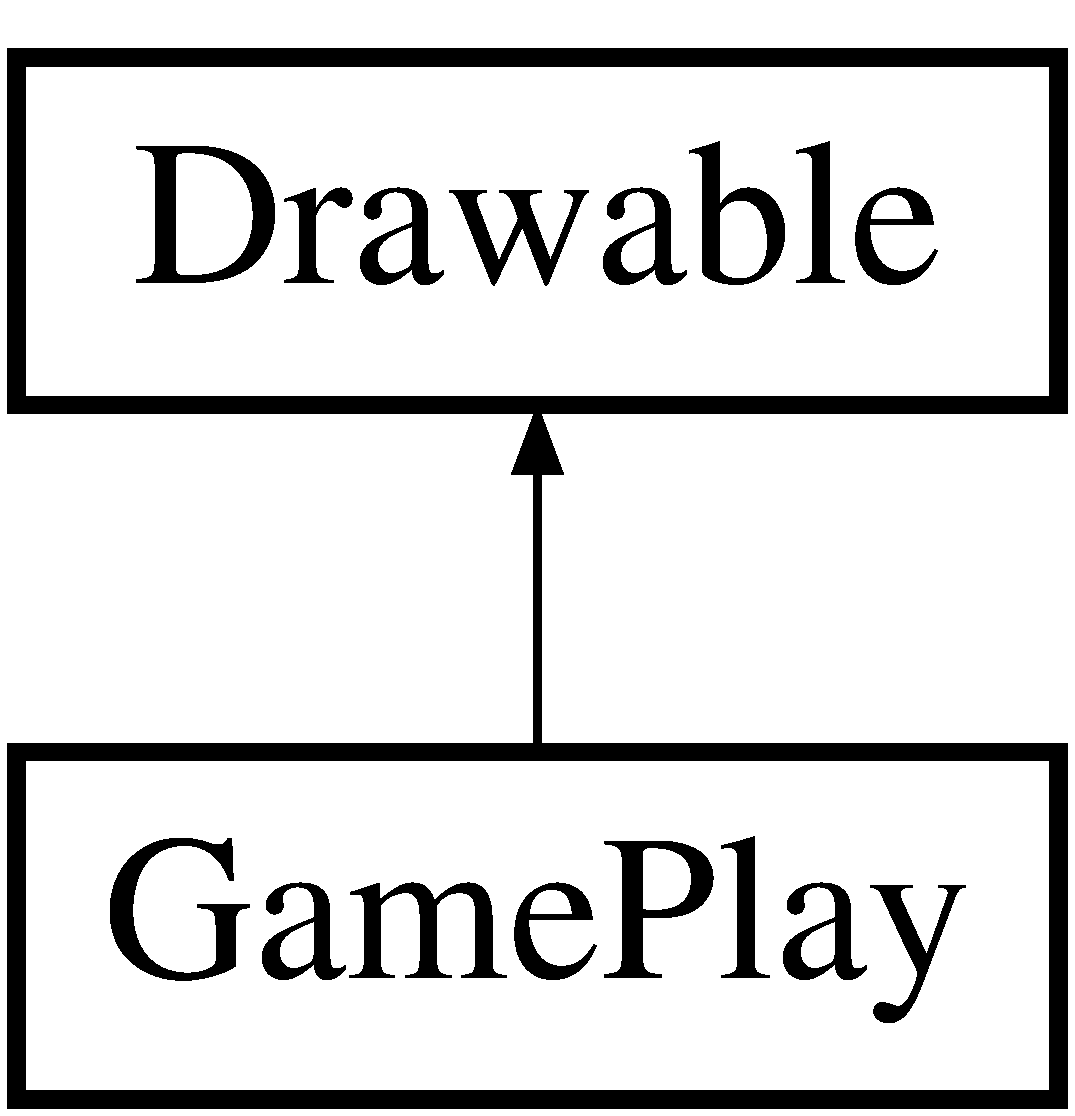
\includegraphics[height=2.000000cm]{class_game_play}
\end{center}
\end{figure}
\subsection*{Public Member Functions}
\begin{DoxyCompactItemize}
\item 
\hypertarget{class_game_play_a3e82b490b9780b0df24a88a9efc6709f}{\hyperlink{class_game_play_a3e82b490b9780b0df24a88a9efc6709f}{Game\-Play} ()}\label{class_game_play_a3e82b490b9780b0df24a88a9efc6709f}

\begin{DoxyCompactList}\small\item\em constructor \end{DoxyCompactList}\item 
void \hyperlink{class_game_play_aeac8436214d80bb44f4a3f41ffed6314}{init} ()
\begin{DoxyCompactList}\small\item\em initialise function \end{DoxyCompactList}\item 
void \hyperlink{class_game_play_a32f780550fae20146e6d6bf844ee3eae}{update} (float time)
\begin{DoxyCompactList}\small\item\em Game update function. \end{DoxyCompactList}\item 
void \hyperlink{class_game_play_adc7a40e331c11d6484b4fe625da96156}{collision\-Handling} ()
\begin{DoxyCompactList}\small\item\em \hyperlink{class_collision}{Collision} handling function. \end{DoxyCompactList}\item 
\hypertarget{class_game_play_aa3e1d8529f943df0a459a08546984681}{virtual void \hyperlink{class_game_play_aa3e1d8529f943df0a459a08546984681}{draw} (sf\-::\-Render\-Target \&target, sf\-::\-Render\-States states) const }\label{class_game_play_aa3e1d8529f943df0a459a08546984681}

\begin{DoxyCompactList}\small\item\em Draw function. \end{DoxyCompactList}\item 
void \hyperlink{class_game_play_a474ed6cf3fcfd1426bfed9c88f24c83c}{screen\-Movement} (\hyperlink{class_player}{Player} \&p, sf\-::\-View \&v, sf\-::\-Sprite \&s)
\begin{DoxyCompactList}\small\item\em function for screen views \end{DoxyCompactList}\item 
void \hyperlink{class_game_play_a8e2237eb9247de338d23c832a7a3e48d}{level\-Finish} (float time)
\begin{DoxyCompactList}\small\item\em Level finish check function. \end{DoxyCompactList}\item 
void \hyperlink{class_game_play_af855db71ec71c4910376ae3cb23fd6fb}{load\-Level} (char $\ast$filename)
\begin{DoxyCompactList}\small\item\em Level loading function. \end{DoxyCompactList}\end{DoxyCompactItemize}
\subsection*{Protected Types}
\begin{DoxyCompactItemize}
\item 
enum {\bfseries Messages} \{ \\*
{\bfseries Title}, 
{\bfseries Lives}, 
{\bfseries Score}, 
{\bfseries Time\-Score}, 
\\*
{\bfseries Final\-Score}
 \}
\end{DoxyCompactItemize}
\subsection*{Protected Attributes}
\begin{DoxyCompactItemize}
\item 
\hyperlink{class_player}{Player} \hyperlink{class_game_play_a08dc6e920f9c76ce54be4e5d2095851b}{player}
\begin{DoxyCompactList}\small\item\em game play variables \end{DoxyCompactList}\item 
\hypertarget{class_game_play_a69aedc07836f2a6630702874e93eec47}{\hyperlink{class_npc}{Npc} \hyperlink{class_game_play_a69aedc07836f2a6630702874e93eec47}{npc\-Holder}}\label{class_game_play_a69aedc07836f2a6630702874e93eec47}

\begin{DoxyCompactList}\small\item\em holder for the npc object \end{DoxyCompactList}\item 
\hypertarget{class_game_play_ab0d25bacfb204bb2afa6763ef9a75ff7}{int \hyperlink{class_game_play_ab0d25bacfb204bb2afa6763ef9a75ff7}{number\-Of\-Npc}}\label{class_game_play_ab0d25bacfb204bb2afa6763ef9a75ff7}

\begin{DoxyCompactList}\small\item\em number of N\-P\-C's in the game \end{DoxyCompactList}\item 
\hypertarget{class_game_play_af6a6d6655b44e08772197ff964992560}{bool \hyperlink{class_game_play_af6a6d6655b44e08772197ff964992560}{in\-Play}}\label{class_game_play_af6a6d6655b44e08772197ff964992560}

\begin{DoxyCompactList}\small\item\em if the game is currently in play \end{DoxyCompactList}\item 
\hypertarget{class_game_play_acbc454f0ef89136874c5cea74064aa6f}{std\-::vector$<$ \hyperlink{class_npc}{Npc} $>$ \hyperlink{class_game_play_acbc454f0ef89136874c5cea74064aa6f}{npc}}\label{class_game_play_acbc454f0ef89136874c5cea74064aa6f}

\begin{DoxyCompactList}\small\item\em vector of N\-P\-C objects \end{DoxyCompactList}\item 
\hypertarget{class_game_play_a8fc2705e520ebb05be8c7e69c318f232}{std\-::vector$<$ \hyperlink{class_npc}{Npc} $>$ \hyperlink{class_game_play_a8fc2705e520ebb05be8c7e69c318f232}{power\-Ups}}\label{class_game_play_a8fc2705e520ebb05be8c7e69c318f232}

\begin{DoxyCompactList}\small\item\em Vector of Power U\-Ps. \end{DoxyCompactList}\item 
\hypertarget{class_game_play_aa33f712517e35db81403bfb7a18ad377}{\hyperlink{class_collision}{Collision} \hyperlink{class_game_play_aa33f712517e35db81403bfb7a18ad377}{collision}}\label{class_game_play_aa33f712517e35db81403bfb7a18ad377}

\begin{DoxyCompactList}\small\item\em \hyperlink{class_collision}{Collision} object. \end{DoxyCompactList}\item 
\hypertarget{class_game_play_abfaadad7bfa0cbb644ff2caf437e97ae}{unsigned int {\bfseries Screen\-Width}}\label{class_game_play_abfaadad7bfa0cbb644ff2caf437e97ae}

\item 
\hypertarget{class_game_play_a56097b45197c2ab545732fc3817bf687}{unsigned int \hyperlink{class_game_play_a56097b45197c2ab545732fc3817bf687}{screen\-Height}}\label{class_game_play_a56097b45197c2ab545732fc3817bf687}

\begin{DoxyCompactList}\small\item\em screen width and screen height \end{DoxyCompactList}\item 
\hypertarget{class_game_play_a1b2dc1f6a0cb155b184f66912ec24fc3}{sf\-::\-Texture \hyperlink{class_game_play_a1b2dc1f6a0cb155b184f66912ec24fc3}{background\-Text}}\label{class_game_play_a1b2dc1f6a0cb155b184f66912ec24fc3}

\begin{DoxyCompactList}\small\item\em background and castle variables \end{DoxyCompactList}\item 
\hypertarget{class_game_play_a851c000ae34c29852abb63379bc02549}{sf\-::\-Sprite {\bfseries background\-Sprite}}\label{class_game_play_a851c000ae34c29852abb63379bc02549}

\item 
\hypertarget{class_game_play_aecfc71ab7e4d1b0625ae8eda94b29f98}{sf\-::\-Texture {\bfseries castle\-Texture}}\label{class_game_play_aecfc71ab7e4d1b0625ae8eda94b29f98}

\item 
\hypertarget{class_game_play_a1bb10da53412b68d2d4f54db073f4d72}{sf\-::\-Sprite {\bfseries castle\-Sprite}}\label{class_game_play_a1bb10da53412b68d2d4f54db073f4d72}

\item 
\hypertarget{class_game_play_a765d7c61edbed2971d63e77e81a89f49}{sf\-::\-Texture {\bfseries shroom\-Text}}\label{class_game_play_a765d7c61edbed2971d63e77e81a89f49}

\item 
\hypertarget{class_game_play_a030b3b8f41d4978c8627dc9c143d7c36}{sf\-::\-Texture {\bfseries star\-Text}}\label{class_game_play_a030b3b8f41d4978c8627dc9c143d7c36}

\item 
\hypertarget{class_game_play_a56313f8852fd827b287dd23042834bbb}{sf\-::\-View \hyperlink{class_game_play_a56313f8852fd827b287dd23042834bbb}{main\-View}}\label{class_game_play_a56313f8852fd827b287dd23042834bbb}

\begin{DoxyCompactList}\small\item\em view variables \end{DoxyCompactList}\item 
\hypertarget{class_game_play_ab8b905f9011ae5eb4084a8c2b71aab86}{sf\-::\-View {\bfseries title\-View}}\label{class_game_play_ab8b905f9011ae5eb4084a8c2b71aab86}

\item 
\hypertarget{class_game_play_a8c84893f2b8892e1a6b14862eab6226a}{sf\-::\-View {\bfseries score\-View}}\label{class_game_play_a8c84893f2b8892e1a6b14862eab6226a}

\item 
\hypertarget{class_game_play_a4fe13e5df316c1653ce9478f6093a18d}{sf\-::\-View {\bfseries lives\-View}}\label{class_game_play_a4fe13e5df316c1653ce9478f6093a18d}

\item 
\hypertarget{class_game_play_aab47a53b15e8fe155e504e45b8dcc86b}{sf\-::\-Font \hyperlink{class_game_play_aab47a53b15e8fe155e504e45b8dcc86b}{S\-M\-Font}}\label{class_game_play_aab47a53b15e8fe155e504e45b8dcc86b}

\begin{DoxyCompactList}\small\item\em text variables \end{DoxyCompactList}\item 
\hypertarget{class_game_play_aedc5312f7a7c45b47340c0860a44dbbd}{sf\-::\-Text {\bfseries message} \mbox{[}5\mbox{]}}\label{class_game_play_aedc5312f7a7c45b47340c0860a44dbbd}

\item 
\hypertarget{class_game_play_afff7c793e76f9f6a96e8db58c15a1537}{int {\bfseries score}}\label{class_game_play_afff7c793e76f9f6a96e8db58c15a1537}

\item 
\hypertarget{class_game_play_a134f4b536cb27725ed3bfffa0da7f4ef}{int {\bfseries lives}}\label{class_game_play_a134f4b536cb27725ed3bfffa0da7f4ef}

\item 
\hypertarget{class_game_play_a32aa78dc4bd232cb1119c66399dcb125}{int {\bfseries time\-Score}}\label{class_game_play_a32aa78dc4bd232cb1119c66399dcb125}

\item 
\hypertarget{class_game_play_a9e2d1f5136cf7eb12d8d7c56d54d3c0b}{int {\bfseries final\-Score}}\label{class_game_play_a9e2d1f5136cf7eb12d8d7c56d54d3c0b}

\item 
\hypertarget{class_game_play_ad3e56c63e9689496eb999bf260d85409}{int {\bfseries level}}\label{class_game_play_ad3e56c63e9689496eb999bf260d85409}

\item 
\hypertarget{class_game_play_a8f3424d1523e4a2be8593883a3fd198f}{std\-::string {\bfseries String\-Message} \mbox{[}5\mbox{]}}\label{class_game_play_a8f3424d1523e4a2be8593883a3fd198f}

\item 
std\-::vector$<$ std\-::vector$<$ int $>$ $>$ \hyperlink{class_game_play_aa8ae61ae157cacf1be80773aa9fde3b0}{layout}
\begin{DoxyCompactList}\small\item\em level loading variables \end{DoxyCompactList}\item 
\hypertarget{class_game_play_a87c503c3b96f4158718e4765d37464ce}{std\-::vector$<$ \hyperlink{class_block}{Block} $>$ \hyperlink{class_game_play_a87c503c3b96f4158718e4765d37464ce}{row\-Vector}}\label{class_game_play_a87c503c3b96f4158718e4765d37464ce}

\begin{DoxyCompactList}\small\item\em 1\-D vector of blocks to load into blocks vector \end{DoxyCompactList}\item 
\hypertarget{class_game_play_a28a01697eaf1aff08b9d7ac0106def07}{std\-::vector$<$ std\-::vector$<$ \hyperlink{class_block}{Block} $>$ $>$ \hyperlink{class_game_play_a28a01697eaf1aff08b9d7ac0106def07}{blocks}}\label{class_game_play_a28a01697eaf1aff08b9d7ac0106def07}

\begin{DoxyCompactList}\small\item\em 2\-D vector of blocks \end{DoxyCompactList}\item 
\hypertarget{class_game_play_a97ddf6ce01d8f315c968136f97fb7ec9}{sf\-::\-Texture {\bfseries floor\-Texture}}\label{class_game_play_a97ddf6ce01d8f315c968136f97fb7ec9}

\item 
\hypertarget{class_game_play_acad50fbec26ac840a3b7a9610eb949f4}{sf\-::\-Texture {\bfseries normal\-Texture}}\label{class_game_play_acad50fbec26ac840a3b7a9610eb949f4}

\item 
\hypertarget{class_game_play_a1bfe51d46513cab9ed1419b51643e77a}{sf\-::\-Texture {\bfseries break\-Texture}}\label{class_game_play_a1bfe51d46513cab9ed1419b51643e77a}

\item 
\hypertarget{class_game_play_a4fd92145ae1d1b65ac4a933ed22855de}{sf\-::\-Texture {\bfseries power\-Up\-Texture}}\label{class_game_play_a4fd92145ae1d1b65ac4a933ed22855de}

\item 
\hypertarget{class_game_play_a9cb665d35b995eb01658b7061dcfd9a2}{sf\-::\-Texture \hyperlink{class_game_play_a9cb665d35b995eb01658b7061dcfd9a2}{used\-Block\-Texture}}\label{class_game_play_a9cb665d35b995eb01658b7061dcfd9a2}

\begin{DoxyCompactList}\small\item\em textures for special objects \end{DoxyCompactList}\item 
\hypertarget{class_game_play_a5e30dd99fa90fd0972f6061b7d96fe44}{int \hyperlink{class_game_play_a5e30dd99fa90fd0972f6061b7d96fe44}{number\-Of\-Blocks}}\label{class_game_play_a5e30dd99fa90fd0972f6061b7d96fe44}

\begin{DoxyCompactList}\small\item\em Number of blocks in the level. \end{DoxyCompactList}\item 
\hypertarget{class_game_play_a46c26ce716c6b1345576ceca7682883e}{float \hyperlink{class_game_play_a46c26ce716c6b1345576ceca7682883e}{block\-Scale}}\label{class_game_play_a46c26ce716c6b1345576ceca7682883e}

\begin{DoxyCompactList}\small\item\em scale of blocks \end{DoxyCompactList}\item 
\hypertarget{class_game_play_af336a085728fd157bb3ddb72a9349ae2}{sf\-::\-Sound\-Buffer \hyperlink{class_game_play_af336a085728fd157bb3ddb72a9349ae2}{backgroundbuffer}}\label{class_game_play_af336a085728fd157bb3ddb72a9349ae2}

\begin{DoxyCompactList}\small\item\em Sound variables. \end{DoxyCompactList}\item 
\hypertarget{class_game_play_adcb91b78525022f0f29ec60fec06faa4}{sf\-::\-Sound\-Buffer {\bfseries game\-Over\-Buffer}}\label{class_game_play_adcb91b78525022f0f29ec60fec06faa4}

\item 
\hypertarget{class_game_play_a82e90b0bfce0443471b54943a11f254d}{sf\-::\-Sound\-Buffer {\bfseries coin\-Buffer}}\label{class_game_play_a82e90b0bfce0443471b54943a11f254d}

\item 
\hypertarget{class_game_play_a086bd4e522cc7f107aa8729da37f0d0f}{sf\-::\-Sound\-Buffer {\bfseries win\-Buffer}}\label{class_game_play_a086bd4e522cc7f107aa8729da37f0d0f}

\item 
\hypertarget{class_game_play_a15bb2d831db86a7cb66fd89568971b63}{sf\-::\-Sound\-Buffer {\bfseries block\-Break\-Buffer}}\label{class_game_play_a15bb2d831db86a7cb66fd89568971b63}

\item 
\hypertarget{class_game_play_ab58ca928fcddef9ce2739ea5b68f074d}{sf\-::\-Sound\-Buffer {\bfseries power\-Up\-Block\-Buffer}}\label{class_game_play_ab58ca928fcddef9ce2739ea5b68f074d}

\item 
\hypertarget{class_game_play_a0954ad834629cf6acb1235562c0e8d79}{sf\-::\-Sound\-Buffer {\bfseries power\-Up\-Buffer}}\label{class_game_play_a0954ad834629cf6acb1235562c0e8d79}

\item 
\hypertarget{class_game_play_a8dad752106ccef7498c8cdec564c3640}{sf\-::\-Sound {\bfseries game\-Over\-Sound}}\label{class_game_play_a8dad752106ccef7498c8cdec564c3640}

\item 
\hypertarget{class_game_play_aff2e8ec6a84bde0974943682715e2ce0}{sf\-::\-Sound {\bfseries coin\-Sound}}\label{class_game_play_aff2e8ec6a84bde0974943682715e2ce0}

\item 
\hypertarget{class_game_play_aca7e389685b4fe52cacd43da0c5f6188}{sf\-::\-Sound {\bfseries win\-Sound}}\label{class_game_play_aca7e389685b4fe52cacd43da0c5f6188}

\item 
\hypertarget{class_game_play_a1c2c6762b82ae0a369403a9902404529}{sf\-::\-Sound {\bfseries block\-Break\-Sound}}\label{class_game_play_a1c2c6762b82ae0a369403a9902404529}

\item 
\hypertarget{class_game_play_a7967804865ed893966d7cda335f255bf}{sf\-::\-Sound {\bfseries power\-Up\-Block\-Sound}}\label{class_game_play_a7967804865ed893966d7cda335f255bf}

\item 
\hypertarget{class_game_play_afd382f7d108792a43e5223e43e498653}{sf\-::\-Sound {\bfseries power\-Up\-Sound}}\label{class_game_play_afd382f7d108792a43e5223e43e498653}

\item 
\hypertarget{class_game_play_a26196da953ca24d8bbd0a669c99777b4}{sf\-::\-Music {\bfseries background\-Music}}\label{class_game_play_a26196da953ca24d8bbd0a669c99777b4}

\end{DoxyCompactItemize}


\subsection{Detailed Description}
the game play events 

\subsection{Member Function Documentation}
\hypertarget{class_game_play_adc7a40e331c11d6484b4fe625da96156}{\index{Game\-Play@{Game\-Play}!collision\-Handling@{collision\-Handling}}
\index{collision\-Handling@{collision\-Handling}!GamePlay@{Game\-Play}}
\subsubsection[{collision\-Handling}]{\setlength{\rightskip}{0pt plus 5cm}void Game\-Play\-::collision\-Handling (
\begin{DoxyParamCaption}
{}
\end{DoxyParamCaption}
)}}\label{class_game_play_adc7a40e331c11d6484b4fe625da96156}


\hyperlink{class_collision}{Collision} handling function. 

\hyperlink{class_collision}{Collision} between npcs and player

$<$ if npc's still exist

$<$ if there is a collision between player and the npc

$<$ calculate collision normal

$<$ if the N\-P\-C is an enemy

$<$ if player lands on top of npc

$<$ resolve collision

$<$ reduce lives by 1

$<$ remove player buffs

$<$ remove player buffs

$<$ change pitch of music back

$<$ reset position of player

$<$ set screen center on player

$<$ if the npc's normal is 1

$<$ make player bounce a little bit

$<$ erase npc from vector

$<$ increase score by 50

$<$ if the N\-P\-C is a shroom

if the player falls down

$<$ reduce lives by 1

$<$ reset players position

$<$ set screen center on player

$<$ remove player buffs

$<$ remove player buffs

$<$ change pitch of music back

$<$ If player has collided with a block

$<$ calculate the collision normal

$<$ resolve the collision

$<$ if the player bounced ontop and the block is destroyable

$<$ and the blocks hits left is 0

$<$ erase block

$<$ grand 25 score

$<$ else reduce hits by 1

$<$ if player hits from underneat on a special block

$<$ change block to be used

$<$ increase score

$<$ set hits left to 0

$<$ if there is a collision between an npc and a block

$<$ calculate collision normal

$<$ resolve the collision

depending on which side the npc hits, change it's velocity \hypertarget{class_game_play_aeac8436214d80bb44f4a3f41ffed6314}{\index{Game\-Play@{Game\-Play}!init@{init}}
\index{init@{init}!GamePlay@{Game\-Play}}
\subsubsection[{init}]{\setlength{\rightskip}{0pt plus 5cm}void Game\-Play\-::init (
\begin{DoxyParamCaption}
{}
\end{DoxyParamCaption}
)}}\label{class_game_play_aeac8436214d80bb44f4a3f41ffed6314}


initialise function 

set the variable in\-Play to be true

Set the required variables for player

load level function to load all the blocks

Create the enemy N\-P\-C's and push them back onto the npc vector

set the N\-P\-C's velocity and playability

load background and finish-\/point castle

Set the main view properties

initialise the messages

load font for text

set font, character size and assign the message string to the variable

position each message on the screen

Initialise the sound variables

Background music

Win Sound

Game Over Sound

Coin Sound

\hyperlink{class_block}{Block} Breaking Sound

Power Up \hyperlink{class_block}{Block} Sound

Power Up Sound

assign remaining game play \hypertarget{class_game_play_a8e2237eb9247de338d23c832a7a3e48d}{\index{Game\-Play@{Game\-Play}!level\-Finish@{level\-Finish}}
\index{level\-Finish@{level\-Finish}!GamePlay@{Game\-Play}}
\subsubsection[{level\-Finish}]{\setlength{\rightskip}{0pt plus 5cm}void Game\-Play\-::level\-Finish (
\begin{DoxyParamCaption}
\item[{float}]{time}
\end{DoxyParamCaption}
)}}\label{class_game_play_a8e2237eb9247de338d23c832a7a3e48d}


Level finish check function. 

$<$ if game is not inplay

$<$ calculate final score

$<$include remaining lives in score

$<$update final score

$<$ if the player reaches the end

$<$ stop the player from moving

$<$ erase the npc vector

$<$ set position of message in correct location

$<$ erase the npc vector

$<$ if the player hits R

$<$ set position of message in correct location

$<$ if the player hits R

$<$ change inplay to be true

$<$ erase the npc vector

$<$ re initialise the game 
\begin{DoxyParams}{Parameters}
{\em time} & level finish function \\
\hline
\end{DoxyParams}
\hypertarget{class_game_play_af855db71ec71c4910376ae3cb23fd6fb}{\index{Game\-Play@{Game\-Play}!load\-Level@{load\-Level}}
\index{load\-Level@{load\-Level}!GamePlay@{Game\-Play}}
\subsubsection[{load\-Level}]{\setlength{\rightskip}{0pt plus 5cm}void Game\-Play\-::load\-Level (
\begin{DoxyParamCaption}
\item[{char $\ast$}]{filename}
\end{DoxyParamCaption}
)}}\label{class_game_play_af855db71ec71c4910376ae3cb23fd6fb}


Level loading function. 

set variables to be 0

$<$ vector for pushing into the 2d Vector \char`\"{}blocks\char`\"{}

$<$ rows and cols

$<$ current block to push into the row vector 
\begin{DoxyParams}{Parameters}
{\em filename} & level loading function \\
\hline
\end{DoxyParams}
\hypertarget{class_game_play_a474ed6cf3fcfd1426bfed9c88f24c83c}{\index{Game\-Play@{Game\-Play}!screen\-Movement@{screen\-Movement}}
\index{screen\-Movement@{screen\-Movement}!GamePlay@{Game\-Play}}
\subsubsection[{screen\-Movement}]{\setlength{\rightskip}{0pt plus 5cm}void Game\-Play\-::screen\-Movement (
\begin{DoxyParamCaption}
\item[{{\bf Player} \&}]{p, }
\item[{sf\-::\-View \&}]{v, }
\item[{sf\-::\-Sprite \&}]{s}
\end{DoxyParamCaption}
)}}\label{class_game_play_a474ed6cf3fcfd1426bfed9c88f24c83c}


function for screen views 

screen move right

screen move left

screen move up

screen move down

keeps background static

keeps messages in place 
\begin{DoxyParams}{Parameters}
{\em s} & screen movement function to keep in track with player \\
\hline
\end{DoxyParams}
\hypertarget{class_game_play_a32f780550fae20146e6d6bf844ee3eae}{\index{Game\-Play@{Game\-Play}!update@{update}}
\index{update@{update}!GamePlay@{Game\-Play}}
\subsubsection[{update}]{\setlength{\rightskip}{0pt plus 5cm}void Game\-Play\-::update (
\begin{DoxyParamCaption}
\item[{float}]{time}
\end{DoxyParamCaption}
)}}\label{class_game_play_a32f780550fae20146e6d6bf844ee3eae}


Game update function. 

Decrease the time bonus score over time

npc update functions

$<$ animate the npc

$<$ integrate the npc

integrate / animate player object

$<$ if game is inplay then the player can move

$<$ collision handling function call

$<$ screen movement function call

update the score messages with the actual score

if player is dead, erase all npc's and run the init function again

level finish function call (checks if level has been complete) 

\subsection{Member Data Documentation}
\hypertarget{class_game_play_aa8ae61ae157cacf1be80773aa9fde3b0}{\index{Game\-Play@{Game\-Play}!layout@{layout}}
\index{layout@{layout}!GamePlay@{Game\-Play}}
\subsubsection[{layout}]{\setlength{\rightskip}{0pt plus 5cm}std\-::vector$<$std\-::vector$<$int$>$ $>$ Game\-Play\-::layout\hspace{0.3cm}{\ttfamily [protected]}}}\label{class_game_play_aa8ae61ae157cacf1be80773aa9fde3b0}


level loading variables 

vector of ints for block layout \hypertarget{class_game_play_a08dc6e920f9c76ce54be4e5d2095851b}{\index{Game\-Play@{Game\-Play}!player@{player}}
\index{player@{player}!GamePlay@{Game\-Play}}
\subsubsection[{player}]{\setlength{\rightskip}{0pt plus 5cm}{\bf Player} Game\-Play\-::player\hspace{0.3cm}{\ttfamily [protected]}}}\label{class_game_play_a08dc6e920f9c76ce54be4e5d2095851b}


game play variables 

player object 

The documentation for this class was generated from the following files\-:\begin{DoxyCompactItemize}
\item 
include/\hyperlink{_game_play_8h}{Game\-Play.\-h}\item 
src/\hyperlink{_game_play_8cpp}{Game\-Play.\-cpp}\end{DoxyCompactItemize}

\hypertarget{class_movable}{\section{Movable Class Reference}
\label{class_movable}\index{Movable@{Movable}}
}


{\ttfamily \#include $<$Movable.\-h$>$}

Inheritance diagram for Movable\-:\begin{figure}[H]
\begin{center}
\leavevmode
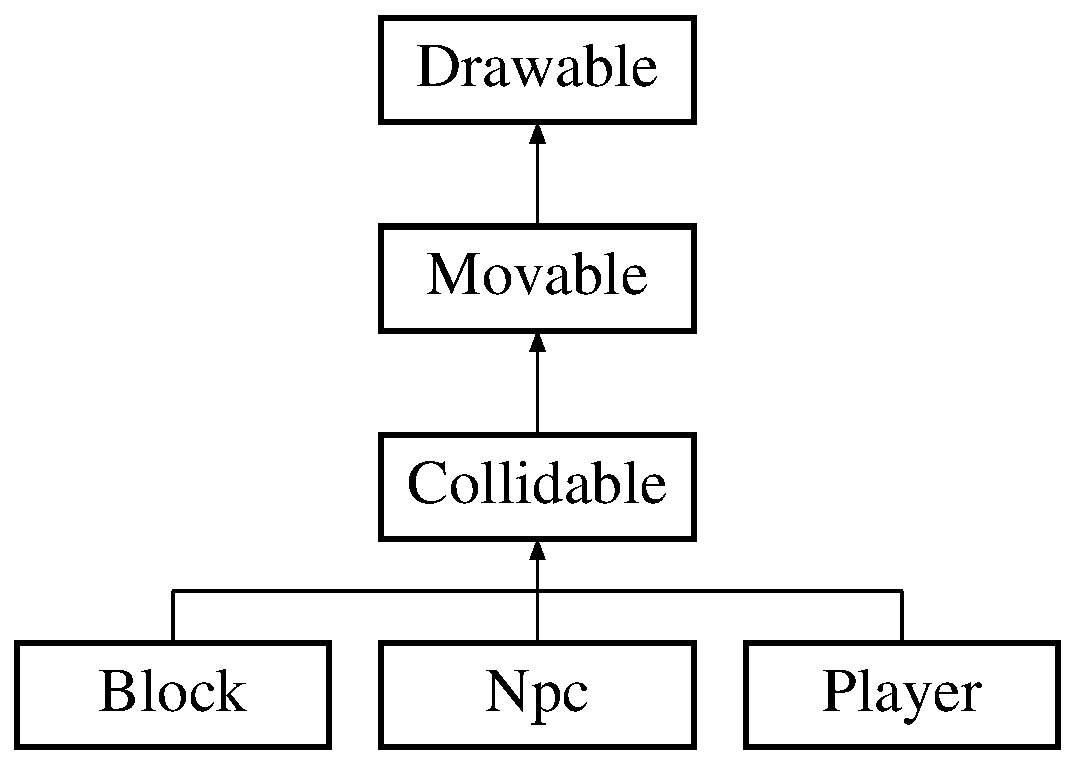
\includegraphics[height=4.000000cm]{class_movable}
\end{center}
\end{figure}
\subsection*{Public Member Functions}
\begin{DoxyCompactItemize}
\item 
\hypertarget{class_movable_a053cf48796f1aef5b6f6cb4c6b22db78}{\hyperlink{class_movable_a053cf48796f1aef5b6f6cb4c6b22db78}{Movable} ()}\label{class_movable_a053cf48796f1aef5b6f6cb4c6b22db78}

\begin{DoxyCompactList}\small\item\em default constructor \end{DoxyCompactList}\item 
void \hyperlink{class_movable_ac7c594e41f6b95e70b0c851dfdf2738a}{init} (\hyperlink{class_vector2_d}{Vector2\-D} \&v, \hyperlink{class_vector2_d}{Vector2\-D} \&p, \hyperlink{class_vector2_d}{Vector2\-D} \&a)
\begin{DoxyCompactList}\small\item\em initialise function \end{DoxyCompactList}\item 
void \hyperlink{class_movable_a3d7bfc8850dade678649be4ebefd38ca}{set\-Pos} (\hyperlink{class_vector2_d}{Vector2\-D} \&pos)
\begin{DoxyCompactList}\small\item\em Position setter. \end{DoxyCompactList}\item 
void \hyperlink{class_movable_ad7eb0895f66e471a5348e1051efb0bc6}{set\-Vel} (\hyperlink{class_vector2_d}{Vector2\-D} \&vel)
\begin{DoxyCompactList}\small\item\em Velocity setter. \end{DoxyCompactList}\item 
void \hyperlink{class_movable_a01eca1584038ac6347b9dd7a5c4d14be}{set\-Acc} (\hyperlink{class_vector2_d}{Vector2\-D} \&acc)
\begin{DoxyCompactList}\small\item\em Acceleration setter. \end{DoxyCompactList}\item 
\hypertarget{class_movable_a62a255d120f31673e6a8021384bfa3ae}{void \hyperlink{class_movable_a62a255d120f31673e6a8021384bfa3ae}{scale\-Sprite} (float sx, float sy)}\label{class_movable_a62a255d120f31673e6a8021384bfa3ae}

\begin{DoxyCompactList}\small\item\em Scale sprite function. \end{DoxyCompactList}\item 
\hypertarget{class_movable_ad8531638ef85fdb7f91f3e596c15275d}{void \hyperlink{class_movable_ad8531638ef85fdb7f91f3e596c15275d}{set\-Playable} (bool p)}\label{class_movable_ad8531638ef85fdb7f91f3e596c15275d}

\begin{DoxyCompactList}\small\item\em set playability of object \end{DoxyCompactList}\item 
\hypertarget{class_movable_ada07aadc68ac39a5252f27c2c25a46bb}{\hyperlink{class_vector2_d}{Vector2\-D} \hyperlink{class_movable_ada07aadc68ac39a5252f27c2c25a46bb}{get\-Pos} ()}\label{class_movable_ada07aadc68ac39a5252f27c2c25a46bb}

\begin{DoxyCompactList}\small\item\em Position getter. \end{DoxyCompactList}\item 
\hypertarget{class_movable_a8c95174062940a2b728218b81881cf62}{\hyperlink{class_vector2_d}{Vector2\-D} \hyperlink{class_movable_a8c95174062940a2b728218b81881cf62}{get\-Vel} ()}\label{class_movable_a8c95174062940a2b728218b81881cf62}

\begin{DoxyCompactList}\small\item\em Velocity getter. \end{DoxyCompactList}\item 
\hypertarget{class_movable_a73d65f64cb2167203ce4a202bc693b27}{\hyperlink{class_vector2_d}{Vector2\-D} \hyperlink{class_movable_a73d65f64cb2167203ce4a202bc693b27}{get\-Acc} ()}\label{class_movable_a73d65f64cb2167203ce4a202bc693b27}

\begin{DoxyCompactList}\small\item\em Acceleration getter. \end{DoxyCompactList}\item 
\hypertarget{class_movable_a3d6756247c44c31646f99c9857ab06c9}{bool \hyperlink{class_movable_a3d6756247c44c31646f99c9857ab06c9}{get\-Playable} ()}\label{class_movable_a3d6756247c44c31646f99c9857ab06c9}

\begin{DoxyCompactList}\small\item\em Getter for the playability bool. \end{DoxyCompactList}\item 
\hypertarget{class_movable_a80af67a0660d45e1088ed344f902ade1}{int \hyperlink{class_movable_a80af67a0660d45e1088ed344f902ade1}{get\-Cols} ()}\label{class_movable_a80af67a0660d45e1088ed344f902ade1}

\begin{DoxyCompactList}\small\item\em Getter for colums in sprite sheet. \end{DoxyCompactList}\item 
\hypertarget{class_movable_a5ca927f75fb88aff35060ea7c3dc057f}{float \hyperlink{class_movable_a5ca927f75fb88aff35060ea7c3dc057f}{get\-Image\-Height} ()}\label{class_movable_a5ca927f75fb88aff35060ea7c3dc057f}

\begin{DoxyCompactList}\small\item\em Getter for images height. \end{DoxyCompactList}\item 
\hypertarget{class_movable_a2fbc46d99e0fde3f8e6f91dee513ae64}{float \hyperlink{class_movable_a2fbc46d99e0fde3f8e6f91dee513ae64}{get\-Image\-Width} ()}\label{class_movable_a2fbc46d99e0fde3f8e6f91dee513ae64}

\begin{DoxyCompactList}\small\item\em Getter for images width. \end{DoxyCompactList}\item 
\hypertarget{class_movable_ab6e4a29915ebae856e3cb74ffa51c66d}{float \hyperlink{class_movable_ab6e4a29915ebae856e3cb74ffa51c66d}{get\-Anim\-Delay} ()}\label{class_movable_ab6e4a29915ebae856e3cb74ffa51c66d}

\begin{DoxyCompactList}\small\item\em Getter for sprites animation delay. \end{DoxyCompactList}\item 
void \hyperlink{class_movable_a48eda08ba135395d3a033ac3bd395d13}{integrate} (float h)
\begin{DoxyCompactList}\small\item\em Integrate function. \end{DoxyCompactList}\item 
void \hyperlink{class_movable_a85b93f096b982eff2683ec3d185bbe35}{set\-Texture} (sf\-::\-Texture t, int columns, float anim\-Delay)
\begin{DoxyCompactList}\small\item\em texture setter \end{DoxyCompactList}\item 
\hypertarget{class_movable_a7a9ea13658207006945ff3d151cf59f7}{void \hyperlink{class_movable_a7a9ea13658207006945ff3d151cf59f7}{animate} ()}\label{class_movable_a7a9ea13658207006945ff3d151cf59f7}

\begin{DoxyCompactList}\small\item\em Animate function. \end{DoxyCompactList}\item 
\hypertarget{class_movable_ac4e1b69e5c6225f138dba25c4d6dd197}{void \hyperlink{class_movable_ac4e1b69e5c6225f138dba25c4d6dd197}{set\-Animate\-Properties} (int columns, int height, int width, float delay)}\label{class_movable_ac4e1b69e5c6225f138dba25c4d6dd197}

\begin{DoxyCompactList}\small\item\em Animation properties setter function. \end{DoxyCompactList}\item 
virtual void \hyperlink{class_movable_aeae46b44643f7c8d9a58bacba683fe7b}{draw} (sf\-::\-Render\-Target \&target, sf\-::\-Render\-States states) const 
\begin{DoxyCompactList}\small\item\em Draw function for objects. \end{DoxyCompactList}\end{DoxyCompactItemize}
\subsection*{Protected Attributes}
\begin{DoxyCompactItemize}
\item 
\hypertarget{class_movable_aabc3da1506fc73517ed6b41de02b8192}{\hyperlink{class_vector2_d}{Vector2\-D} \hyperlink{class_movable_aabc3da1506fc73517ed6b41de02b8192}{position}}\label{class_movable_aabc3da1506fc73517ed6b41de02b8192}

\begin{DoxyCompactList}\small\item\em \hyperlink{class_vector2_d}{Vector2\-D} of position. \end{DoxyCompactList}\item 
\hypertarget{class_movable_afc13818f829b2b2fd6319f3c2b8ad2df}{\hyperlink{class_vector2_d}{Vector2\-D} \hyperlink{class_movable_afc13818f829b2b2fd6319f3c2b8ad2df}{velocity}}\label{class_movable_afc13818f829b2b2fd6319f3c2b8ad2df}

\begin{DoxyCompactList}\small\item\em \hyperlink{class_vector2_d}{Vector2\-D} of velocity. \end{DoxyCompactList}\item 
\hypertarget{class_movable_a1e5dd5fb67401d0692cfcba4d1dc371d}{\hyperlink{class_vector2_d}{Vector2\-D} \hyperlink{class_movable_a1e5dd5fb67401d0692cfcba4d1dc371d}{acceleration}}\label{class_movable_a1e5dd5fb67401d0692cfcba4d1dc371d}

\begin{DoxyCompactList}\small\item\em \hyperlink{class_vector2_d}{Vector2\-D} of acceleration. \end{DoxyCompactList}\item 
\hypertarget{class_movable_a4391fef1d549bb6f91bf8943bc11d395}{\hyperlink{class_vector2_d}{Vector2\-D} \hyperlink{class_movable_a4391fef1d549bb6f91bf8943bc11d395}{drag}}\label{class_movable_a4391fef1d549bb6f91bf8943bc11d395}

\begin{DoxyCompactList}\small\item\em \hyperlink{class_vector2_d}{Vector2\-D} of drag. \end{DoxyCompactList}\item 
\hypertarget{class_movable_affaa847aef26cd4268ecf12bf28e2950}{\hyperlink{class_vector2_d}{Vector2\-D} \hyperlink{class_movable_affaa847aef26cd4268ecf12bf28e2950}{max\-Velocity}}\label{class_movable_affaa847aef26cd4268ecf12bf28e2950}

\begin{DoxyCompactList}\small\item\em Max velocity variable as a 2\-D Vector. \end{DoxyCompactList}\item 
\hypertarget{class_movable_a33f5b527f0ef2d47360c1c5d5d3b02b4}{sf\-::\-Sprite \hyperlink{class_movable_a33f5b527f0ef2d47360c1c5d5d3b02b4}{move\-Sprite}}\label{class_movable_a33f5b527f0ef2d47360c1c5d5d3b02b4}

\begin{DoxyCompactList}\small\item\em sprite of movable object \end{DoxyCompactList}\item 
\hypertarget{class_movable_a9c521594c4b5d7b4f597a05940839674}{bool \hyperlink{class_movable_a9c521594c4b5d7b4f597a05940839674}{playable}}\label{class_movable_a9c521594c4b5d7b4f597a05940839674}

\begin{DoxyCompactList}\small\item\em Is object playable. \end{DoxyCompactList}\item 
\hypertarget{class_movable_a629fcd93be7b4c904b151d4dcfab28d6}{sf\-::\-Clock \hyperlink{class_movable_a629fcd93be7b4c904b151d4dcfab28d6}{animation\-Clock}}\label{class_movable_a629fcd93be7b4c904b151d4dcfab28d6}

\begin{DoxyCompactList}\small\item\em a clock shared by all animations \end{DoxyCompactList}\item 
\hypertarget{class_movable_a7b884da4aa6fc964a8708b08639c63a8}{int \hyperlink{class_movable_a7b884da4aa6fc964a8708b08639c63a8}{count}}\label{class_movable_a7b884da4aa6fc964a8708b08639c63a8}

\begin{DoxyCompactList}\small\item\em animation count \end{DoxyCompactList}\item 
\hypertarget{class_movable_adcb7431454605451f9b36432d1efc957}{double {\bfseries last\-Time}}\label{class_movable_adcb7431454605451f9b36432d1efc957}

\item 
\hypertarget{class_movable_afe64fcc8c67accc7bdc25370b5c2d90d}{sf\-::\-Int\-Rect \hyperlink{class_movable_afe64fcc8c67accc7bdc25370b5c2d90d}{r}}\label{class_movable_afe64fcc8c67accc7bdc25370b5c2d90d}

\begin{DoxyCompactList}\small\item\em texture rect for animation \end{DoxyCompactList}\item 
\hypertarget{class_movable_a5eafe8f13e492e43b47d5a97d85badcb}{int \hyperlink{class_movable_a5eafe8f13e492e43b47d5a97d85badcb}{cols}}\label{class_movable_a5eafe8f13e492e43b47d5a97d85badcb}

\begin{DoxyCompactList}\small\item\em Columns for animation. \end{DoxyCompactList}\item 
\hypertarget{class_movable_a0935c58ae1e43d05d6a3887c947d7f7e}{float {\bfseries image\-Height}}\label{class_movable_a0935c58ae1e43d05d6a3887c947d7f7e}

\item 
\hypertarget{class_movable_a4383f3e3c5f60088838458d05b4b9c48}{float {\bfseries image\-Width}}\label{class_movable_a4383f3e3c5f60088838458d05b4b9c48}

\item 
\hypertarget{class_movable_a9dec862effcc876c6f1500fa214bc550}{float \hyperlink{class_movable_a9dec862effcc876c6f1500fa214bc550}{tile\-Width}}\label{class_movable_a9dec862effcc876c6f1500fa214bc550}

\begin{DoxyCompactList}\small\item\em stores texture height and width for animation \end{DoxyCompactList}\item 
\hypertarget{class_movable_a2f7229b260b7b6282a262dca99fc6770}{float \hyperlink{class_movable_a2f7229b260b7b6282a262dca99fc6770}{animation\-Delay}}\label{class_movable_a2f7229b260b7b6282a262dca99fc6770}

\begin{DoxyCompactList}\small\item\em delay for animation sequence \end{DoxyCompactList}\item 
\hypertarget{class_movable_a2d7847d46b685a3d873afec5be1adddc}{bool \hyperlink{class_movable_a2d7847d46b685a3d873afec5be1adddc}{animating}}\label{class_movable_a2d7847d46b685a3d873afec5be1adddc}

\begin{DoxyCompactList}\small\item\em check if object is currently in animation \end{DoxyCompactList}\end{DoxyCompactItemize}


\subsection{Detailed Description}
for all the movable objects in the game  position/velocity/acceleration etc. 

\subsection{Member Function Documentation}
\hypertarget{class_movable_aeae46b44643f7c8d9a58bacba683fe7b}{\index{Movable@{Movable}!draw@{draw}}
\index{draw@{draw}!Movable@{Movable}}
\subsubsection[{draw}]{\setlength{\rightskip}{0pt plus 5cm}void Movable\-::draw (
\begin{DoxyParamCaption}
\item[{sf\-::\-Render\-Target \&}]{target, }
\item[{sf\-::\-Render\-States}]{states}
\end{DoxyParamCaption}
) const\hspace{0.3cm}{\ttfamily [virtual]}}}\label{class_movable_aeae46b44643f7c8d9a58bacba683fe7b}


Draw function for objects. 

$<$ Draw function for objects \hypertarget{class_movable_ac7c594e41f6b95e70b0c851dfdf2738a}{\index{Movable@{Movable}!init@{init}}
\index{init@{init}!Movable@{Movable}}
\subsubsection[{init}]{\setlength{\rightskip}{0pt plus 5cm}void Movable\-::init (
\begin{DoxyParamCaption}
\item[{{\bf Vector2\-D} \&}]{v, }
\item[{{\bf Vector2\-D} \&}]{p, }
\item[{{\bf Vector2\-D} \&}]{a}
\end{DoxyParamCaption}
)}}\label{class_movable_ac7c594e41f6b95e70b0c851dfdf2738a}


initialise function 


\begin{DoxyParams}{Parameters}
{\em a} & initialise function \\
\hline
\end{DoxyParams}
\hypertarget{class_movable_a48eda08ba135395d3a033ac3bd395d13}{\index{Movable@{Movable}!integrate@{integrate}}
\index{integrate@{integrate}!Movable@{Movable}}
\subsubsection[{integrate}]{\setlength{\rightskip}{0pt plus 5cm}void Movable\-::integrate (
\begin{DoxyParamCaption}
\item[{float}]{h}
\end{DoxyParamCaption}
)}}\label{class_movable_a48eda08ba135395d3a033ac3bd395d13}


Integrate function. 

$<$ if the object is playable

$<$ calculate drage

improved euler for movement 
\begin{DoxyParams}{Parameters}
{\em h} & Integrate function \\
\hline
\end{DoxyParams}
\hypertarget{class_movable_a01eca1584038ac6347b9dd7a5c4d14be}{\index{Movable@{Movable}!set\-Acc@{set\-Acc}}
\index{set\-Acc@{set\-Acc}!Movable@{Movable}}
\subsubsection[{set\-Acc}]{\setlength{\rightskip}{0pt plus 5cm}void Movable\-::set\-Acc (
\begin{DoxyParamCaption}
\item[{{\bf Vector2\-D} \&}]{acc}
\end{DoxyParamCaption}
)}}\label{class_movable_a01eca1584038ac6347b9dd7a5c4d14be}


Acceleration setter. 


\begin{DoxyParams}{Parameters}
{\em acc} & Acceleration setter \\
\hline
\end{DoxyParams}
\hypertarget{class_movable_a3d7bfc8850dade678649be4ebefd38ca}{\index{Movable@{Movable}!set\-Pos@{set\-Pos}}
\index{set\-Pos@{set\-Pos}!Movable@{Movable}}
\subsubsection[{set\-Pos}]{\setlength{\rightskip}{0pt plus 5cm}void Movable\-::set\-Pos (
\begin{DoxyParamCaption}
\item[{{\bf Vector2\-D} \&}]{pos}
\end{DoxyParamCaption}
)}}\label{class_movable_a3d7bfc8850dade678649be4ebefd38ca}


Position setter. 


\begin{DoxyParams}{Parameters}
{\em pos} & Position setter \\
\hline
\end{DoxyParams}
\hypertarget{class_movable_a85b93f096b982eff2683ec3d185bbe35}{\index{Movable@{Movable}!set\-Texture@{set\-Texture}}
\index{set\-Texture@{set\-Texture}!Movable@{Movable}}
\subsubsection[{set\-Texture}]{\setlength{\rightskip}{0pt plus 5cm}void Movable\-::set\-Texture (
\begin{DoxyParamCaption}
\item[{sf\-::\-Texture}]{t, }
\item[{int}]{columns, }
\item[{float}]{anim\-Delay}
\end{DoxyParamCaption}
)}}\label{class_movable_a85b93f096b982eff2683ec3d185bbe35}


texture setter 

$<$ sets texture rect, and all other required properties for animation 
\begin{DoxyParams}{Parameters}
{\em anim\-Delay} & texture setter \\
\hline
\end{DoxyParams}
\hypertarget{class_movable_ad7eb0895f66e471a5348e1051efb0bc6}{\index{Movable@{Movable}!set\-Vel@{set\-Vel}}
\index{set\-Vel@{set\-Vel}!Movable@{Movable}}
\subsubsection[{set\-Vel}]{\setlength{\rightskip}{0pt plus 5cm}void Movable\-::set\-Vel (
\begin{DoxyParamCaption}
\item[{{\bf Vector2\-D} \&}]{vel}
\end{DoxyParamCaption}
)}}\label{class_movable_ad7eb0895f66e471a5348e1051efb0bc6}


Velocity setter. 


\begin{DoxyParams}{Parameters}
{\em vel} & Velocity setter \\
\hline
\end{DoxyParams}


The documentation for this class was generated from the following files\-:\begin{DoxyCompactItemize}
\item 
include/\hyperlink{_movable_8h}{Movable.\-h}\item 
src/\hyperlink{_movable_8cpp}{Movable.\-cpp}\end{DoxyCompactItemize}

\hypertarget{class_npc}{\section{Npc Class Reference}
\label{class_npc}\index{Npc@{Npc}}
}


{\ttfamily \#include $<$Npc.\-h$>$}

Inheritance diagram for Npc\-:\begin{figure}[H]
\begin{center}
\leavevmode
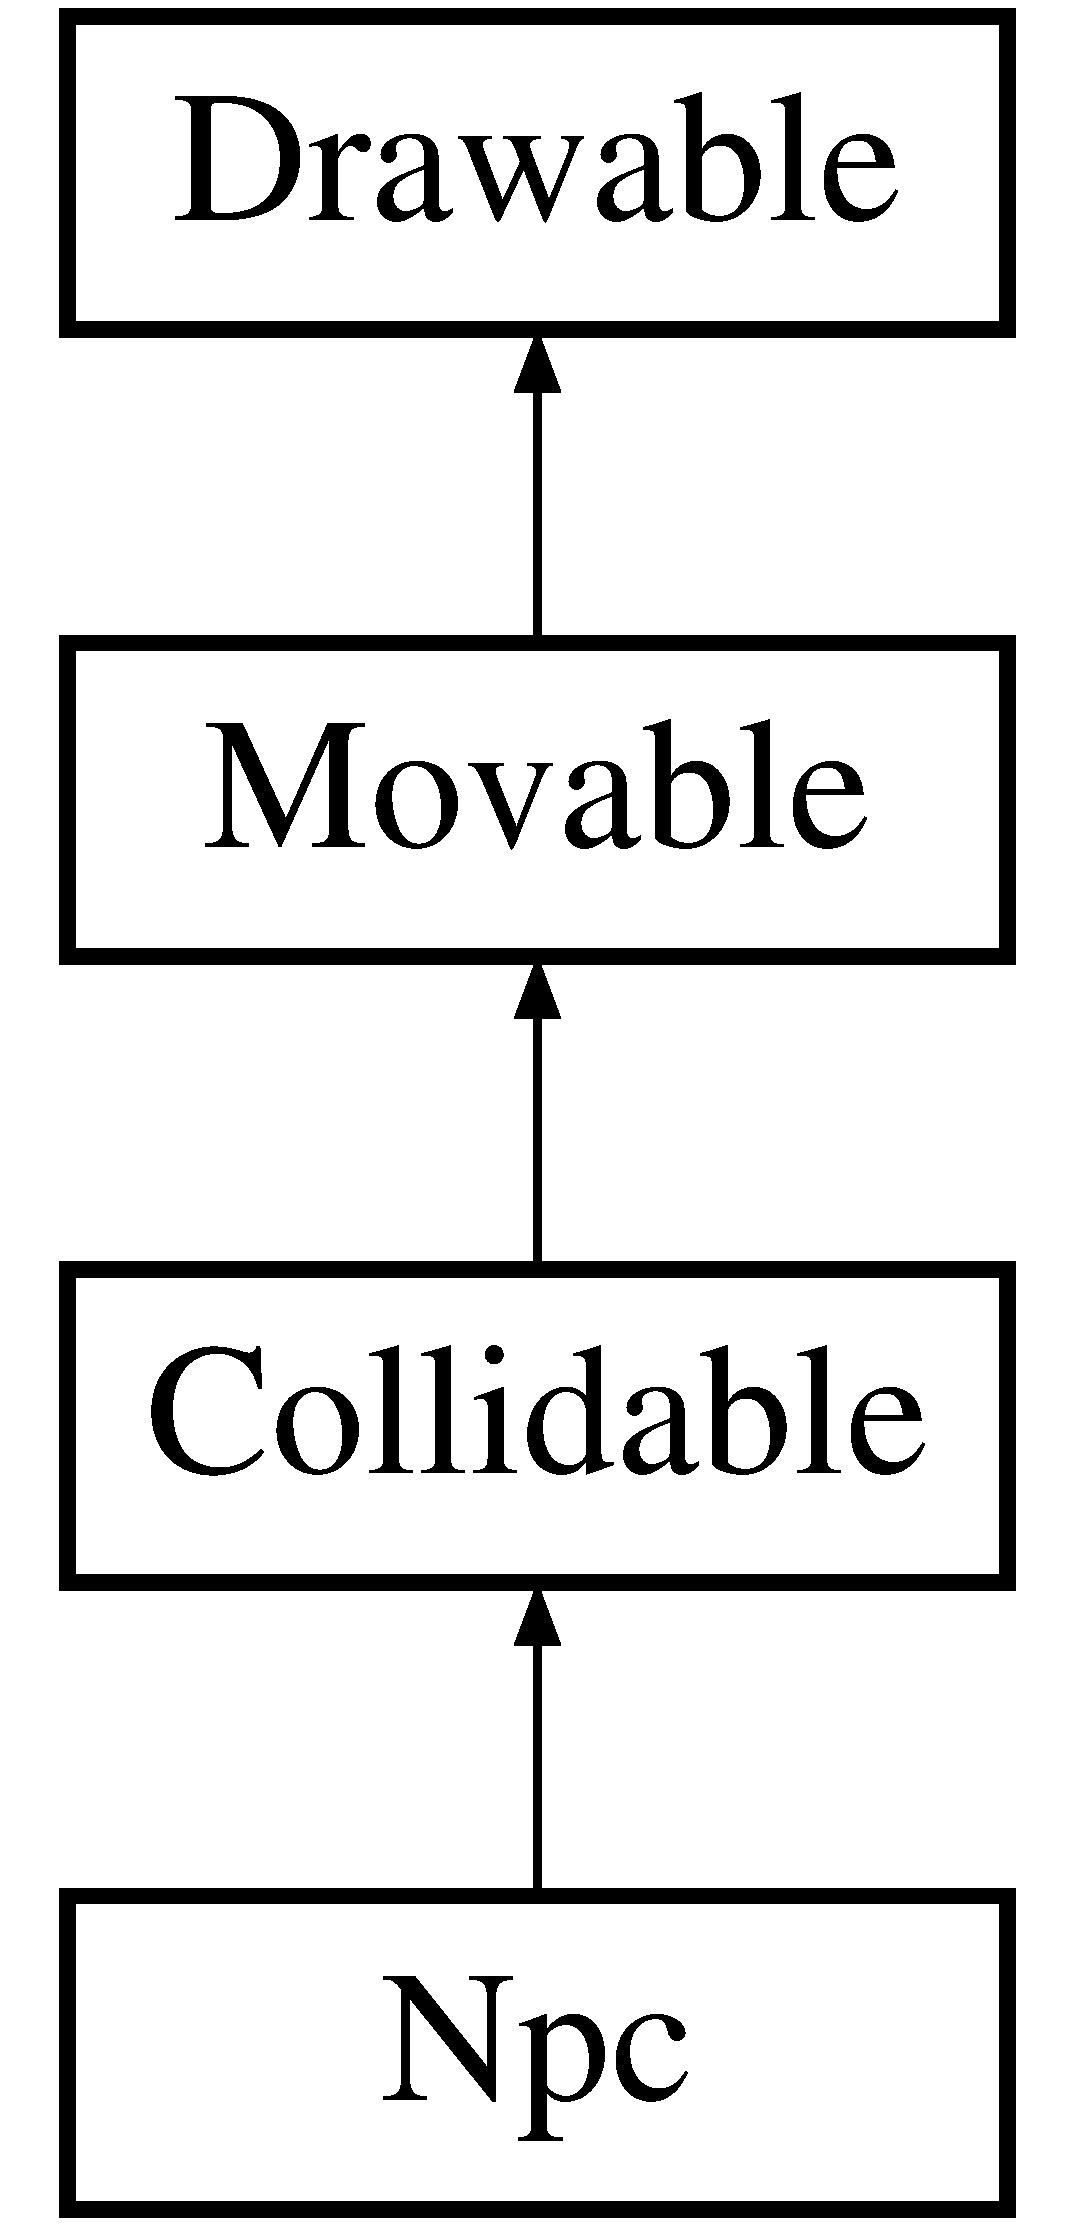
\includegraphics[height=4.000000cm]{class_npc}
\end{center}
\end{figure}
\subsection*{Public Member Functions}
\begin{DoxyCompactItemize}
\item 
\hyperlink{class_npc_a748bee1d096f0dc38a80f2db64186644}{Npc} ()
\item 
void \hyperlink{class_npc_a37c66a6ffa287ad975f42c1ab1d65310}{rand\-Enemy} ()
\begin{DoxyCompactList}\small\item\em Create a random enemy. \end{DoxyCompactList}\item 
void \hyperlink{class_npc_a8ab8f95be18d4add56959b2620e51a2b}{rand\-Power\-Up} (sf\-::\-Texture \&t)
\begin{DoxyCompactList}\small\item\em Create a random power up. \end{DoxyCompactList}\item 
\hypertarget{class_npc_aade5b490d2e23a8a53af6f44c1fc1905}{bool \hyperlink{class_npc_aade5b490d2e23a8a53af6f44c1fc1905}{get\-Direction} ()}\label{class_npc_aade5b490d2e23a8a53af6f44c1fc1905}

\begin{DoxyCompactList}\small\item\em Get the direction the N\-P\-C is facing. \end{DoxyCompactList}\item 
\hypertarget{class_npc_aa2e93dd316c37c06205bcc90027b8c73}{int {\bfseries get\-Power\-U\-P\-Num} ()}\label{class_npc_aa2e93dd316c37c06205bcc90027b8c73}

\end{DoxyCompactItemize}
\subsection*{Protected Types}
\begin{DoxyCompactItemize}
\item 
enum {\bfseries npc\-Type} \{ {\bfseries Goomba}, 
{\bfseries koopa}
 \}
\item 
enum {\bfseries power\-Up\-Type} \{ {\bfseries shroom}, 
{\bfseries star}
 \}
\end{DoxyCompactItemize}
\subsection*{Protected Attributes}
\begin{DoxyCompactItemize}
\item 
\hypertarget{class_npc_ad1ad29ff396ef6164c8ccaecaefa5f5b}{sf\-::\-Texture {\bfseries Goomba\-Text}}\label{class_npc_ad1ad29ff396ef6164c8ccaecaefa5f5b}

\item 
\hypertarget{class_npc_a1eb1469869b587c975379feede8a3fb6}{sf\-::\-Texture {\bfseries koopa\-Left\-Text}}\label{class_npc_a1eb1469869b587c975379feede8a3fb6}

\item 
\hypertarget{class_npc_a1e75f38ac92cba55f14379b97f8f64b4}{sf\-::\-Texture \hyperlink{class_npc_a1e75f38ac92cba55f14379b97f8f64b4}{koopa\-Right\-Text}}\label{class_npc_a1e75f38ac92cba55f14379b97f8f64b4}

\begin{DoxyCompactList}\small\item\em enemy textures \end{DoxyCompactList}\item 
\hypertarget{class_npc_aabe6a589907a40e8955fc79bed1082d9}{sf\-::\-Texture {\bfseries shroom\-Text}}\label{class_npc_aabe6a589907a40e8955fc79bed1082d9}

\item 
\hypertarget{class_npc_a33b0a408e5908f550c30d9802980b0c3}{sf\-::\-Texture \hyperlink{class_npc_a33b0a408e5908f550c30d9802980b0c3}{star\-Text}}\label{class_npc_a33b0a408e5908f550c30d9802980b0c3}

\begin{DoxyCompactList}\small\item\em Power up textures. \end{DoxyCompactList}\item 
\hypertarget{class_npc_aa8b57395241330993689a8839a820b98}{bool \hyperlink{class_npc_aa8b57395241330993689a8839a820b98}{direction}}\label{class_npc_aa8b57395241330993689a8839a820b98}

\begin{DoxyCompactList}\small\item\em direction (left == false, right == true); \end{DoxyCompactList}\item 
\hypertarget{class_npc_a5afc655bd1418b0a489f0ca9da47e560}{int \hyperlink{class_npc_a5afc655bd1418b0a489f0ca9da47e560}{power\-Up\-Num}}\label{class_npc_a5afc655bd1418b0a489f0ca9da47e560}

\begin{DoxyCompactList}\small\item\em number to check if npc is a power up, 0 = no power up, 1 = shroom, 2 = star \end{DoxyCompactList}\end{DoxyCompactItemize}


\subsection{Detailed Description}
for non playable characters and powerups  powerup to be an N\-P\-C as it moves as well. 

\subsection{Constructor \& Destructor Documentation}
\hypertarget{class_npc_a748bee1d096f0dc38a80f2db64186644}{\index{Npc@{Npc}!Npc@{Npc}}
\index{Npc@{Npc}!Npc@{Npc}}
\subsubsection[{Npc}]{\setlength{\rightskip}{0pt plus 5cm}Npc\-::\-Npc (
\begin{DoxyParamCaption}
{}
\end{DoxyParamCaption}
)}}\label{class_npc_a748bee1d096f0dc38a80f2db64186644}
load all the textures from files 

\subsection{Member Function Documentation}
\hypertarget{class_npc_a37c66a6ffa287ad975f42c1ab1d65310}{\index{Npc@{Npc}!rand\-Enemy@{rand\-Enemy}}
\index{rand\-Enemy@{rand\-Enemy}!Npc@{Npc}}
\subsubsection[{rand\-Enemy}]{\setlength{\rightskip}{0pt plus 5cm}void Npc\-::rand\-Enemy (
\begin{DoxyParamCaption}
{}
\end{DoxyParamCaption}
)}}\label{class_npc_a37c66a6ffa287ad975f42c1ab1d65310}


Create a random enemy. 

create Goomba

create Koopa

set animation properties \hypertarget{class_npc_a8ab8f95be18d4add56959b2620e51a2b}{\index{Npc@{Npc}!rand\-Power\-Up@{rand\-Power\-Up}}
\index{rand\-Power\-Up@{rand\-Power\-Up}!Npc@{Npc}}
\subsubsection[{rand\-Power\-Up}]{\setlength{\rightskip}{0pt plus 5cm}void Npc\-::rand\-Power\-Up (
\begin{DoxyParamCaption}
\item[{sf\-::\-Texture \&}]{t}
\end{DoxyParamCaption}
)}}\label{class_npc_a8ab8f95be18d4add56959b2620e51a2b}


Create a random power up. 

set animation properties 

The documentation for this class was generated from the following files\-:\begin{DoxyCompactItemize}
\item 
include/\hyperlink{_npc_8h}{Npc.\-h}\item 
src/Npc.\-cpp\end{DoxyCompactItemize}

\hypertarget{class_player}{\section{Player Class Reference}
\label{class_player}\index{Player@{Player}}
}


{\ttfamily \#include $<$Player.\-h$>$}

Inheritance diagram for Player\-:\begin{figure}[H]
\begin{center}
\leavevmode
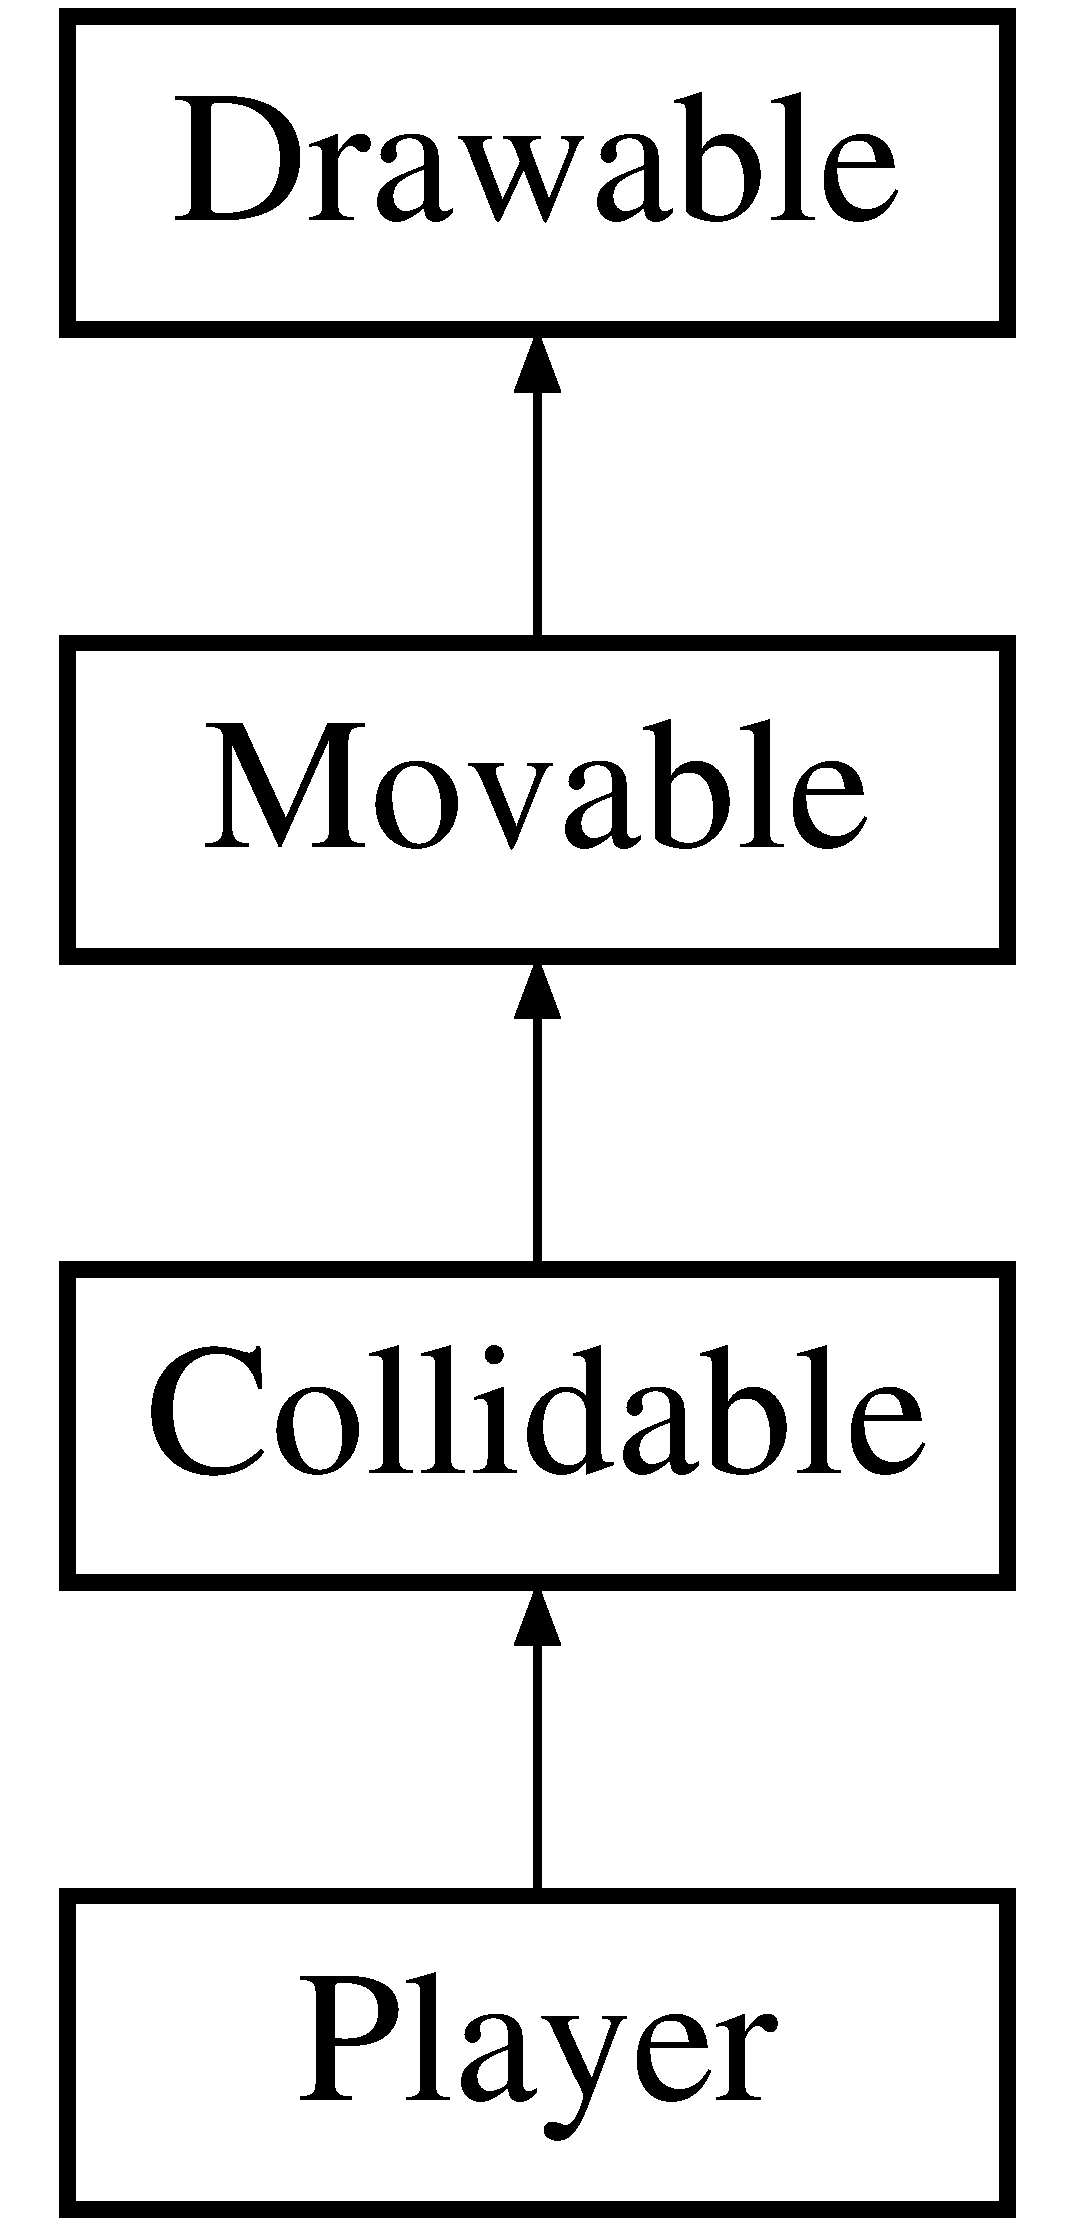
\includegraphics[height=4.000000cm]{class_player}
\end{center}
\end{figure}
\subsection*{Public Member Functions}
\begin{DoxyCompactItemize}
\item 
\hyperlink{class_player_affe0cc3cb714f6deb4e62f0c0d3f1fd8}{Player} ()
\begin{DoxyCompactList}\small\item\em default constructor \end{DoxyCompactList}\item 
void \hyperlink{class_player_a3c2e7e40fe2018229d44168bd484c182}{handle\-Input} ()
\begin{DoxyCompactList}\small\item\em function for handling the input of the player \end{DoxyCompactList}\item 
\hypertarget{class_player_a12121c992641a4f456e5546b735c070e}{void \hyperlink{class_player_a12121c992641a4f456e5546b735c070e}{set\-Buff} (int b, bool t)}\label{class_player_a12121c992641a4f456e5546b735c070e}

\begin{DoxyCompactList}\small\item\em function to set the players buff -\/ integer for which buff and bool on or off \end{DoxyCompactList}\item 
\hypertarget{class_player_af4ff40310af95ecbd9ba06b2108793a3}{int \hyperlink{class_player_af4ff40310af95ecbd9ba06b2108793a3}{get\-Buff} ()}\label{class_player_af4ff40310af95ecbd9ba06b2108793a3}

\begin{DoxyCompactList}\small\item\em returns what type of buff player has -\/ 0 = none, 1 = shroom, 2 = star \end{DoxyCompactList}\end{DoxyCompactItemize}
\subsection*{Protected Types}
\begin{DoxyCompactItemize}
\item 
enum {\bfseries Direction} \{ \\*
{\bfseries left}, 
{\bfseries right}, 
{\bfseries jump}, 
{\bfseries still}, 
\\*
{\bfseries crouch}
 \}
\end{DoxyCompactItemize}
\subsection*{Protected Attributes}
\begin{DoxyCompactItemize}
\item 
\hypertarget{class_player_a5696d1d82851cd6dfd5dbe68b76bfdb1}{sf\-::\-Texture {\bfseries left\-Text}}\label{class_player_a5696d1d82851cd6dfd5dbe68b76bfdb1}

\item 
\hypertarget{class_player_a75ea81350746d65f2290eb487ed648e3}{sf\-::\-Texture {\bfseries right\-Text}}\label{class_player_a75ea81350746d65f2290eb487ed648e3}

\item 
\hypertarget{class_player_a304268d8b7f798b2970f815a33d8abe5}{sf\-::\-Texture {\bfseries jump\-Text}}\label{class_player_a304268d8b7f798b2970f815a33d8abe5}

\item 
\hypertarget{class_player_a5a930a925138d2fbaae4b1da90fb6894}{sf\-::\-Texture {\bfseries still\-Text}}\label{class_player_a5a930a925138d2fbaae4b1da90fb6894}

\item 
\hypertarget{class_player_aac16f632a3e1a8de17e9c8769edf207b}{sf\-::\-Texture \hyperlink{class_player_aac16f632a3e1a8de17e9c8769edf207b}{crouch\-Text}}\label{class_player_aac16f632a3e1a8de17e9c8769edf207b}

\begin{DoxyCompactList}\small\item\em different player textures \end{DoxyCompactList}\item 
\hypertarget{class_player_a93eaebe50e6ab8a19c35138b4c60f60c}{bool \hyperlink{class_player_a93eaebe50e6ab8a19c35138b4c60f60c}{playing}}\label{class_player_a93eaebe50e6ab8a19c35138b4c60f60c}

\begin{DoxyCompactList}\small\item\em is player playing \end{DoxyCompactList}\item 
\hypertarget{class_player_ad50788f8294f0f7acfd03f056f460679}{sf\-::\-Sound\-Buffer \hyperlink{class_player_ad50788f8294f0f7acfd03f056f460679}{soundbuffer}}\label{class_player_ad50788f8294f0f7acfd03f056f460679}

\begin{DoxyCompactList}\small\item\em buffer for jump sound \end{DoxyCompactList}\item 
\hypertarget{class_player_a350d742a163059759e74da611545aa32}{sf\-::\-Sound \hyperlink{class_player_a350d742a163059759e74da611545aa32}{jump\-Sound}}\label{class_player_a350d742a163059759e74da611545aa32}

\begin{DoxyCompactList}\small\item\em jump sound \end{DoxyCompactList}\item 
\hypertarget{class_player_a5991e5d8296b585cdd13bc6c22f40f23}{bool {\bfseries star\-Buff}}\label{class_player_a5991e5d8296b585cdd13bc6c22f40f23}

\item 
\hypertarget{class_player_a2487d863fc3d90ad6bac8cd273136e0f}{bool \hyperlink{class_player_a2487d863fc3d90ad6bac8cd273136e0f}{shroom\-Buff}}\label{class_player_a2487d863fc3d90ad6bac8cd273136e0f}

\begin{DoxyCompactList}\small\item\em if the player has a powerup \end{DoxyCompactList}\end{DoxyCompactItemize}


\subsection{Detailed Description}
\textbackslash{} 

\subsection{Constructor \& Destructor Documentation}
\hypertarget{class_player_affe0cc3cb714f6deb4e62f0c0d3f1fd8}{\index{Player@{Player}!Player@{Player}}
\index{Player@{Player}!Player@{Player}}
\subsubsection[{Player}]{\setlength{\rightskip}{0pt plus 5cm}Player\-::\-Player (
\begin{DoxyParamCaption}
{}
\end{DoxyParamCaption}
)}}\label{class_player_affe0cc3cb714f6deb4e62f0c0d3f1fd8}


default constructor 

set players basic properties

load textures from file

Load the sound for jumping

set the sprites texture and scale

set image height/width and size (for collision and animation)

more properties for animation 

\subsection{Member Function Documentation}
\hypertarget{class_player_a3c2e7e40fe2018229d44168bd484c182}{\index{Player@{Player}!handle\-Input@{handle\-Input}}
\index{handle\-Input@{handle\-Input}!Player@{Player}}
\subsubsection[{handle\-Input}]{\setlength{\rightskip}{0pt plus 5cm}void Player\-::handle\-Input (
\begin{DoxyParamCaption}
{}
\end{DoxyParamCaption}
)}}\label{class_player_a3c2e7e40fe2018229d44168bd484c182}


function for handling the input of the player 

Function handles all player input Changes velocity on key-\/press Changes the texture and animation properties depending on which key you press

$<$ if player pushes right

$<$ change velocity

$<$ change velocity

$<$ set texture to be right

$<$ set animate properties of new texture

$<$ set animating to be true 

The documentation for this class was generated from the following files\-:\begin{DoxyCompactItemize}
\item 
include/\hyperlink{_player_8h}{Player.\-h}\item 
src/\hyperlink{_player_8cpp}{Player.\-cpp}\end{DoxyCompactItemize}

\hypertarget{class_vector2_d}{\section{Vector2\-D Class Reference}
\label{class_vector2_d}\index{Vector2\-D@{Vector2\-D}}
}


{\ttfamily \#include $<$Vector2\-D.\-h$>$}

\subsection*{Public Member Functions}
\begin{DoxyCompactItemize}
\item 
\hypertarget{class_vector2_d_a98e9997ebb7a629f4db52397d4e0d653}{\hyperlink{class_vector2_d_a98e9997ebb7a629f4db52397d4e0d653}{Vector2\-D} ()}\label{class_vector2_d_a98e9997ebb7a629f4db52397d4e0d653}

\begin{DoxyCompactList}\small\item\em Default constructor, set everything to zero. \end{DoxyCompactList}\item 
\hyperlink{class_vector2_d_ab32b5621c9d3b67d506aa3170a789259}{Vector2\-D} (float all\-Values)
\begin{DoxyCompactList}\small\item\em Construtor taking a single value and making all component equal to that value. \end{DoxyCompactList}\item 
\hyperlink{class_vector2_d_a166ca1df158a260a7cbf3b57ff147a4a}{Vector2\-D} (float x, float y)
\begin{DoxyCompactList}\small\item\em Constructor taking x \& y values. \end{DoxyCompactList}\item 
float \hyperlink{class_vector2_d_a4cbde94a1519f61733c607967fa39084}{angle} (\hyperlink{class_vector2_d}{Vector2\-D} \&other)
\begin{DoxyCompactList}\small\item\em angle between this vector and other \end{DoxyCompactList}\item 
float \hyperlink{class_vector2_d_a4b4331ddc82ab81b6e5a66bd861cb315}{dot\-Product} (\hyperlink{class_vector2_d}{Vector2\-D} \&other)
\begin{DoxyCompactList}\small\item\em Returns the dot product of this vector with other. \end{DoxyCompactList}\item 
\hypertarget{class_vector2_d_a007279b304311011d2dc60e940060d30}{\hyperlink{class_vector2_d}{Vector2\-D} \hyperlink{class_vector2_d_a007279b304311011d2dc60e940060d30}{cross\-Product} (\hyperlink{class_vector2_d}{Vector2\-D} \&other)}\label{class_vector2_d_a007279b304311011d2dc60e940060d30}

\begin{DoxyCompactList}\small\item\em Returns the cross product of this vector with other. \end{DoxyCompactList}\item 
\hypertarget{class_vector2_d_a9ec064ffe930ae93d0f420390be126e8}{\hyperlink{class_vector2_d}{Vector2\-D} \hyperlink{class_vector2_d_a9ec064ffe930ae93d0f420390be126e8}{get\-Unit\-Vector} ()}\label{class_vector2_d_a9ec064ffe930ae93d0f420390be126e8}

\begin{DoxyCompactList}\small\item\em Returns the unit vector of this vector. \end{DoxyCompactList}\item 
\hypertarget{class_vector2_d_a527601e47976bcfdac2520817bfee675}{float \hyperlink{class_vector2_d_a527601e47976bcfdac2520817bfee675}{get\-X} ()}\label{class_vector2_d_a527601e47976bcfdac2520817bfee675}

\begin{DoxyCompactList}\small\item\em Returns the X component of this vector. \end{DoxyCompactList}\item 
\hypertarget{class_vector2_d_a5b797fb62a3c21ced0cc8e27afd62f8b}{float \hyperlink{class_vector2_d_a5b797fb62a3c21ced0cc8e27afd62f8b}{get\-Y} ()}\label{class_vector2_d_a5b797fb62a3c21ced0cc8e27afd62f8b}

\begin{DoxyCompactList}\small\item\em Returns the Y component of this vector. \end{DoxyCompactList}\item 
\hypertarget{class_vector2_d_ac458bd997d2f0c6c7234cf1e8a7b73b8}{void \hyperlink{class_vector2_d_ac458bd997d2f0c6c7234cf1e8a7b73b8}{set\-X} (float x)}\label{class_vector2_d_ac458bd997d2f0c6c7234cf1e8a7b73b8}

\begin{DoxyCompactList}\small\item\em set the x component of the vector \end{DoxyCompactList}\item 
\hypertarget{class_vector2_d_a9b47adcbdf2c10f3ba893285b5c34709}{void \hyperlink{class_vector2_d_a9b47adcbdf2c10f3ba893285b5c34709}{set\-Y} (float y)}\label{class_vector2_d_a9b47adcbdf2c10f3ba893285b5c34709}

\begin{DoxyCompactList}\small\item\em set the y component of the vector \end{DoxyCompactList}\item 
\hypertarget{class_vector2_d_a2840db6c516580a39fd5a309d991dae2}{float \hyperlink{class_vector2_d_a2840db6c516580a39fd5a309d991dae2}{magnitude} ()}\label{class_vector2_d_a2840db6c516580a39fd5a309d991dae2}

\begin{DoxyCompactList}\small\item\em Returns the magnitude of this vector. \end{DoxyCompactList}\item 
\hyperlink{class_vector2_d}{Vector2\-D} \hyperlink{class_vector2_d_a07a043fc63572c1cf3104ec0a9a4e796}{operator-\/} (const \hyperlink{class_vector2_d}{Vector2\-D} \&other)
\begin{DoxyCompactList}\small\item\em Component wise subtraction. \end{DoxyCompactList}\item 
\hyperlink{class_vector2_d}{Vector2\-D} \hyperlink{class_vector2_d_a2bed654f65df8c3bedbf8cd7d07071df}{operator+} (const \hyperlink{class_vector2_d}{Vector2\-D} \&other)
\begin{DoxyCompactList}\small\item\em Component wise addition. \end{DoxyCompactList}\item 
\hyperlink{class_vector2_d}{Vector2\-D} \hyperlink{class_vector2_d_a93aad0fe6040d4bde0c7dd3906f6cf90}{operator$\ast$} (const \hyperlink{class_vector2_d}{Vector2\-D} \&other)
\begin{DoxyCompactList}\small\item\em Component wise multiplication. \end{DoxyCompactList}\item 
\hyperlink{class_vector2_d}{Vector2\-D} \hyperlink{class_vector2_d_af509f754de79142227f10cdf7db52fb7}{operator$\ast$} (const float scalar)
\begin{DoxyCompactList}\small\item\em Component wise scalar multiplication. \end{DoxyCompactList}\item 
\hypertarget{class_vector2_d_a7e260b0a6fc69f2c4688a74c641bc68a}{\hyperlink{class_vector2_d}{Vector2\-D} \hyperlink{class_vector2_d_a7e260b0a6fc69f2c4688a74c641bc68a}{operator/} (const float scalar)}\label{class_vector2_d_a7e260b0a6fc69f2c4688a74c641bc68a}

\begin{DoxyCompactList}\small\item\em Component wise scalar division. \end{DoxyCompactList}\end{DoxyCompactItemize}
\subsection*{Protected Attributes}
\begin{DoxyCompactItemize}
\item 
\hypertarget{class_vector2_d_a590d08ddc1841715b476e4876fce3d63}{float \hyperlink{class_vector2_d_a590d08ddc1841715b476e4876fce3d63}{data} \mbox{[}2\mbox{]}}\label{class_vector2_d_a590d08ddc1841715b476e4876fce3d63}

\begin{DoxyCompactList}\small\item\em Data held by the vector. \end{DoxyCompactList}\end{DoxyCompactItemize}


\subsection{Detailed Description}
{\itshape 2\-D} vector 

\subsection{Constructor \& Destructor Documentation}
\hypertarget{class_vector2_d_ab32b5621c9d3b67d506aa3170a789259}{\index{Vector2\-D@{Vector2\-D}!Vector2\-D@{Vector2\-D}}
\index{Vector2\-D@{Vector2\-D}!Vector2D@{Vector2\-D}}
\subsubsection[{Vector2\-D}]{\setlength{\rightskip}{0pt plus 5cm}Vector2\-D\-::\-Vector2\-D (
\begin{DoxyParamCaption}
\item[{float}]{all\-Values}
\end{DoxyParamCaption}
)}}\label{class_vector2_d_ab32b5621c9d3b67d506aa3170a789259}


Construtor taking a single value and making all component equal to that value. 


\begin{DoxyParams}{Parameters}
{\em all\-Values} & Construtor taking a single value and making all component equal to that value \\
\hline
\end{DoxyParams}
\hypertarget{class_vector2_d_a166ca1df158a260a7cbf3b57ff147a4a}{\index{Vector2\-D@{Vector2\-D}!Vector2\-D@{Vector2\-D}}
\index{Vector2\-D@{Vector2\-D}!Vector2D@{Vector2\-D}}
\subsubsection[{Vector2\-D}]{\setlength{\rightskip}{0pt plus 5cm}Vector2\-D\-::\-Vector2\-D (
\begin{DoxyParamCaption}
\item[{float}]{x, }
\item[{float}]{y}
\end{DoxyParamCaption}
)}}\label{class_vector2_d_a166ca1df158a260a7cbf3b57ff147a4a}


Constructor taking x \& y values. 


\begin{DoxyParams}{Parameters}
{\em y} & Constructor taking x and y values \\
\hline
\end{DoxyParams}


\subsection{Member Function Documentation}
\hypertarget{class_vector2_d_a4cbde94a1519f61733c607967fa39084}{\index{Vector2\-D@{Vector2\-D}!angle@{angle}}
\index{angle@{angle}!Vector2D@{Vector2\-D}}
\subsubsection[{angle}]{\setlength{\rightskip}{0pt plus 5cm}float Vector2\-D\-::angle (
\begin{DoxyParamCaption}
\item[{{\bf Vector2\-D} \&}]{other}
\end{DoxyParamCaption}
)}}\label{class_vector2_d_a4cbde94a1519f61733c607967fa39084}


angle between this vector and other 


\begin{DoxyParams}{Parameters}
{\em other} & angle between this vector and other \\
\hline
\end{DoxyParams}
\hypertarget{class_vector2_d_a4b4331ddc82ab81b6e5a66bd861cb315}{\index{Vector2\-D@{Vector2\-D}!dot\-Product@{dot\-Product}}
\index{dot\-Product@{dot\-Product}!Vector2D@{Vector2\-D}}
\subsubsection[{dot\-Product}]{\setlength{\rightskip}{0pt plus 5cm}float Vector2\-D\-::dot\-Product (
\begin{DoxyParamCaption}
\item[{{\bf Vector2\-D} \&}]{other}
\end{DoxyParamCaption}
)}}\label{class_vector2_d_a4b4331ddc82ab81b6e5a66bd861cb315}


Returns the dot product of this vector with other. 


\begin{DoxyParams}{Parameters}
{\em other} & Returns the dot product of this vector with other \\
\hline
\end{DoxyParams}
\hypertarget{class_vector2_d_a93aad0fe6040d4bde0c7dd3906f6cf90}{\index{Vector2\-D@{Vector2\-D}!operator$\ast$@{operator$\ast$}}
\index{operator$\ast$@{operator$\ast$}!Vector2D@{Vector2\-D}}
\subsubsection[{operator$\ast$}]{\setlength{\rightskip}{0pt plus 5cm}{\bf Vector2\-D} Vector2\-D\-::operator$\ast$ (
\begin{DoxyParamCaption}
\item[{const {\bf Vector2\-D} \&}]{other}
\end{DoxyParamCaption}
)}}\label{class_vector2_d_a93aad0fe6040d4bde0c7dd3906f6cf90}


Component wise multiplication. 


\begin{DoxyParams}{Parameters}
{\em other} & Component wise multiplication \\
\hline
\end{DoxyParams}
\hypertarget{class_vector2_d_af509f754de79142227f10cdf7db52fb7}{\index{Vector2\-D@{Vector2\-D}!operator$\ast$@{operator$\ast$}}
\index{operator$\ast$@{operator$\ast$}!Vector2D@{Vector2\-D}}
\subsubsection[{operator$\ast$}]{\setlength{\rightskip}{0pt plus 5cm}{\bf Vector2\-D} Vector2\-D\-::operator$\ast$ (
\begin{DoxyParamCaption}
\item[{const float}]{scalar}
\end{DoxyParamCaption}
)}}\label{class_vector2_d_af509f754de79142227f10cdf7db52fb7}


Component wise scalar multiplication. 


\begin{DoxyParams}{Parameters}
{\em scalar} & Component wise scalar multiplication \\
\hline
\end{DoxyParams}
\hypertarget{class_vector2_d_a2bed654f65df8c3bedbf8cd7d07071df}{\index{Vector2\-D@{Vector2\-D}!operator+@{operator+}}
\index{operator+@{operator+}!Vector2D@{Vector2\-D}}
\subsubsection[{operator+}]{\setlength{\rightskip}{0pt plus 5cm}{\bf Vector2\-D} Vector2\-D\-::operator+ (
\begin{DoxyParamCaption}
\item[{const {\bf Vector2\-D} \&}]{other}
\end{DoxyParamCaption}
)}}\label{class_vector2_d_a2bed654f65df8c3bedbf8cd7d07071df}


Component wise addition. 


\begin{DoxyParams}{Parameters}
{\em other} & Component wise addition \\
\hline
\end{DoxyParams}
\hypertarget{class_vector2_d_a07a043fc63572c1cf3104ec0a9a4e796}{\index{Vector2\-D@{Vector2\-D}!operator-\/@{operator-\/}}
\index{operator-\/@{operator-\/}!Vector2D@{Vector2\-D}}
\subsubsection[{operator-\/}]{\setlength{\rightskip}{0pt plus 5cm}{\bf Vector2\-D} Vector2\-D\-::operator-\/ (
\begin{DoxyParamCaption}
\item[{const {\bf Vector2\-D} \&}]{other}
\end{DoxyParamCaption}
)}}\label{class_vector2_d_a07a043fc63572c1cf3104ec0a9a4e796}


Component wise subtraction. 


\begin{DoxyParams}{Parameters}
{\em other} & Component wise subtraction \\
\hline
\end{DoxyParams}


The documentation for this class was generated from the following files\-:\begin{DoxyCompactItemize}
\item 
include/\hyperlink{_vector2_d_8h}{Vector2\-D.\-h}\item 
src/\hyperlink{_vector2_d_8cpp}{Vector2\-D.\-cpp}\end{DoxyCompactItemize}

\chapter{File Documentation}
\hypertarget{_block_8h}{\section{include/\-Block.h File Reference}
\label{_block_8h}\index{include/\-Block.\-h@{include/\-Block.\-h}}
}
{\ttfamily \#include \char`\"{}Collidable.\-h\char`\"{}}\\*
\subsection*{Classes}
\begin{DoxyCompactItemize}
\item 
class \hyperlink{class_block}{Block}
\end{DoxyCompactItemize}

\hypertarget{_collidable_8h}{\section{include/\-Collidable.h File Reference}
\label{_collidable_8h}\index{include/\-Collidable.\-h@{include/\-Collidable.\-h}}
}
{\ttfamily \#include \char`\"{}Movable.\-h\char`\"{}}\\*
\subsection*{Classes}
\begin{DoxyCompactItemize}
\item 
class \hyperlink{class_collidable}{Collidable}
\end{DoxyCompactItemize}

\hypertarget{_collision_8h}{\section{include/\-Collision.h File Reference}
\label{_collision_8h}\index{include/\-Collision.\-h@{include/\-Collision.\-h}}
}
{\ttfamily \#include \char`\"{}Collidable.\-h\char`\"{}}\\*
{\ttfamily \#include $<$Math.\-h$>$}\\*
{\ttfamily \#include $<$algorithm$>$}\\*
\subsection*{Classes}
\begin{DoxyCompactItemize}
\item 
class \hyperlink{class_collision}{Collision}
\end{DoxyCompactItemize}

\hypertarget{_game_play_8h}{\section{include/\-Game\-Play.h File Reference}
\label{_game_play_8h}\index{include/\-Game\-Play.\-h@{include/\-Game\-Play.\-h}}
}
{\ttfamily \#include $<$S\-F\-M\-L/\-Graphics.\-hpp$>$}\\*
{\ttfamily \#include $<$S\-F\-M\-L/\-Audio.\-hpp$>$}\\*
{\ttfamily \#include $<$fstream$>$}\\*
{\ttfamily \#include $<$sstream$>$}\\*
{\ttfamily \#include $<$iostream$>$}\\*
{\ttfamily \#include \char`\"{}Player.\-h\char`\"{}}\\*
{\ttfamily \#include \char`\"{}Npc.\-h\char`\"{}}\\*
{\ttfamily \#include \char`\"{}Block.\-h\char`\"{}}\\*
{\ttfamily \#include \char`\"{}Collision.\-h\char`\"{}}\\*
\subsection*{Classes}
\begin{DoxyCompactItemize}
\item 
class \hyperlink{class_game_play}{Game\-Play}
\end{DoxyCompactItemize}

\hypertarget{_movable_8h}{\section{include/\-Movable.h File Reference}
\label{_movable_8h}\index{include/\-Movable.\-h@{include/\-Movable.\-h}}
}
{\ttfamily \#include $<$S\-F\-M\-L/\-Graphics.\-hpp$>$}\\*
{\ttfamily \#include \char`\"{}Vector2\-D.\-h\char`\"{}}\\*
{\ttfamily \#include $<$iostream$>$}\\*
\subsection*{Classes}
\begin{DoxyCompactItemize}
\item 
class \hyperlink{class_movable}{Movable}
\end{DoxyCompactItemize}

\hypertarget{_npc_8h}{\section{include/\-Npc.h File Reference}
\label{_npc_8h}\index{include/\-Npc.\-h@{include/\-Npc.\-h}}
}
{\ttfamily \#include \char`\"{}Collidable.\-h\char`\"{}}\\*
\subsection*{Classes}
\begin{DoxyCompactItemize}
\item 
class \hyperlink{class_npc}{Npc}
\end{DoxyCompactItemize}

\hypertarget{_player_8h}{\section{include/\-Player.h File Reference}
\label{_player_8h}\index{include/\-Player.\-h@{include/\-Player.\-h}}
}
{\ttfamily \#include \char`\"{}Collidable.\-h\char`\"{}}\\*
{\ttfamily \#include $<$S\-F\-M\-L/\-Audio.\-hpp$>$}\\*
\subsection*{Classes}
\begin{DoxyCompactItemize}
\item 
class \hyperlink{class_player}{Player}
\end{DoxyCompactItemize}

\hypertarget{_vector2_d_8h}{\section{include/\-Vector2\-D.h File Reference}
\label{_vector2_d_8h}\index{include/\-Vector2\-D.\-h@{include/\-Vector2\-D.\-h}}
}
{\ttfamily \#include $<$cmath$>$}\\*
{\ttfamily \#include $<$cstdlib$>$}\\*
\subsection*{Classes}
\begin{DoxyCompactItemize}
\item 
class \hyperlink{class_vector2_d}{Vector2\-D}
\end{DoxyCompactItemize}

\hypertarget{_collidable_8cpp}{\section{src/\-Collidable.cpp File Reference}
\label{_collidable_8cpp}\index{src/\-Collidable.\-cpp@{src/\-Collidable.\-cpp}}
}
{\ttfamily \#include \char`\"{}Collidable.\-h\char`\"{}}\\*

\hypertarget{_game_play_8cpp}{\section{src/\-Game\-Play.cpp File Reference}
\label{_game_play_8cpp}\index{src/\-Game\-Play.\-cpp@{src/\-Game\-Play.\-cpp}}
}
{\ttfamily \#include \char`\"{}Game\-Play.\-h\char`\"{}}\\*
{\ttfamily \#include $<$iostream$>$}\\*
\subsection*{Functions}
\begin{DoxyCompactItemize}
\item 
\hypertarget{_game_play_8cpp_a3576342d8d20886b8896d957b37721e4}{void {\bfseries screen\-Movement} (\hyperlink{class_movable}{Movable} \&p, sf\-::\-View \&v, sf\-::\-Sprite \&s)}\label{_game_play_8cpp_a3576342d8d20886b8896d957b37721e4}

\end{DoxyCompactItemize}

\hypertarget{_movable_8cpp}{\section{src/\-Movable.cpp File Reference}
\label{_movable_8cpp}\index{src/\-Movable.\-cpp@{src/\-Movable.\-cpp}}
}
{\ttfamily \#include \char`\"{}Movable.\-h\char`\"{}}\\*

\hypertarget{_player_8cpp}{\section{src/\-Player.cpp File Reference}
\label{_player_8cpp}\index{src/\-Player.\-cpp@{src/\-Player.\-cpp}}
}
{\ttfamily \#include \char`\"{}Player.\-h\char`\"{}}\\*

\hypertarget{_vector2_d_8cpp}{\section{src/\-Vector2\-D.cpp File Reference}
\label{_vector2_d_8cpp}\index{src/\-Vector2\-D.\-cpp@{src/\-Vector2\-D.\-cpp}}
}
{\ttfamily \#include \char`\"{}Vector2\-D.\-h\char`\"{}}\\*
{\ttfamily \#include $<$iostream$>$}\\*

%--- End generated contents ---

% Index
\newpage
\phantomsection
\addcontentsline{toc}{part}{Index}
\printindex

\end{document}
